% Options for packages loaded elsewhere
\PassOptionsToPackage{unicode}{hyperref}
\PassOptionsToPackage{hyphens}{url}
\PassOptionsToPackage{dvipsnames,svgnames,x11names}{xcolor}
%
\documentclass[
  ignorenonframetext,
]{beamer}
\usepackage{pgfpages}
\setbeamertemplate{caption}[numbered]
\setbeamertemplate{caption label separator}{: }
\setbeamercolor{caption name}{fg=normal text.fg}
\beamertemplatenavigationsymbolsempty
% Prevent slide breaks in the middle of a paragraph
\widowpenalties 1 10000
\raggedbottom

\usepackage{amsmath,amssymb}
\usepackage{iftex}
\ifPDFTeX
  \usepackage[T1]{fontenc}
  \usepackage[utf8]{inputenc}
  \usepackage{textcomp} % provide euro and other symbols
\else % if luatex or xetex
  \usepackage{unicode-math}
  \defaultfontfeatures{Scale=MatchLowercase}
  \defaultfontfeatures[\rmfamily]{Ligatures=TeX,Scale=1}
\fi
\usepackage{lmodern}
\usetheme[]{AnnArbor}
\usecolortheme{dolphin}
\usefonttheme{structurebold}
\ifPDFTeX\else  
    % xetex/luatex font selection
\fi
% Use upquote if available, for straight quotes in verbatim environments
\IfFileExists{upquote.sty}{\usepackage{upquote}}{}
\IfFileExists{microtype.sty}{% use microtype if available
  \usepackage[]{microtype}
  \UseMicrotypeSet[protrusion]{basicmath} % disable protrusion for tt fonts
}{}
\makeatletter
\@ifundefined{KOMAClassName}{% if non-KOMA class
  \IfFileExists{parskip.sty}{%
    \usepackage{parskip}
  }{% else
    \setlength{\parindent}{0pt}
    \setlength{\parskip}{6pt plus 2pt minus 1pt}}
}{% if KOMA class
  \KOMAoptions{parskip=half}}
\makeatother
\usepackage{xcolor}
\newif\ifbibliography
\setlength{\emergencystretch}{3em} % prevent overfull lines
\setcounter{secnumdepth}{-\maxdimen} % remove section numbering

\usepackage{color}
\usepackage{fancyvrb}
\newcommand{\VerbBar}{|}
\newcommand{\VERB}{\Verb[commandchars=\\\{\}]}
\DefineVerbatimEnvironment{Highlighting}{Verbatim}{commandchars=\\\{\}}
% Add ',fontsize=\small' for more characters per line
\usepackage{framed}
\definecolor{shadecolor}{RGB}{241,243,245}
\newenvironment{Shaded}{\begin{snugshade}}{\end{snugshade}}
\newcommand{\AlertTok}[1]{\textcolor[rgb]{0.68,0.00,0.00}{#1}}
\newcommand{\AnnotationTok}[1]{\textcolor[rgb]{0.37,0.37,0.37}{#1}}
\newcommand{\AttributeTok}[1]{\textcolor[rgb]{0.40,0.45,0.13}{#1}}
\newcommand{\BaseNTok}[1]{\textcolor[rgb]{0.68,0.00,0.00}{#1}}
\newcommand{\BuiltInTok}[1]{\textcolor[rgb]{0.00,0.23,0.31}{#1}}
\newcommand{\CharTok}[1]{\textcolor[rgb]{0.13,0.47,0.30}{#1}}
\newcommand{\CommentTok}[1]{\textcolor[rgb]{0.37,0.37,0.37}{#1}}
\newcommand{\CommentVarTok}[1]{\textcolor[rgb]{0.37,0.37,0.37}{\textit{#1}}}
\newcommand{\ConstantTok}[1]{\textcolor[rgb]{0.56,0.35,0.01}{#1}}
\newcommand{\ControlFlowTok}[1]{\textcolor[rgb]{0.00,0.23,0.31}{\textbf{#1}}}
\newcommand{\DataTypeTok}[1]{\textcolor[rgb]{0.68,0.00,0.00}{#1}}
\newcommand{\DecValTok}[1]{\textcolor[rgb]{0.68,0.00,0.00}{#1}}
\newcommand{\DocumentationTok}[1]{\textcolor[rgb]{0.37,0.37,0.37}{\textit{#1}}}
\newcommand{\ErrorTok}[1]{\textcolor[rgb]{0.68,0.00,0.00}{#1}}
\newcommand{\ExtensionTok}[1]{\textcolor[rgb]{0.00,0.23,0.31}{#1}}
\newcommand{\FloatTok}[1]{\textcolor[rgb]{0.68,0.00,0.00}{#1}}
\newcommand{\FunctionTok}[1]{\textcolor[rgb]{0.28,0.35,0.67}{#1}}
\newcommand{\ImportTok}[1]{\textcolor[rgb]{0.00,0.46,0.62}{#1}}
\newcommand{\InformationTok}[1]{\textcolor[rgb]{0.37,0.37,0.37}{#1}}
\newcommand{\KeywordTok}[1]{\textcolor[rgb]{0.00,0.23,0.31}{\textbf{#1}}}
\newcommand{\NormalTok}[1]{\textcolor[rgb]{0.00,0.23,0.31}{#1}}
\newcommand{\OperatorTok}[1]{\textcolor[rgb]{0.37,0.37,0.37}{#1}}
\newcommand{\OtherTok}[1]{\textcolor[rgb]{0.00,0.23,0.31}{#1}}
\newcommand{\PreprocessorTok}[1]{\textcolor[rgb]{0.68,0.00,0.00}{#1}}
\newcommand{\RegionMarkerTok}[1]{\textcolor[rgb]{0.00,0.23,0.31}{#1}}
\newcommand{\SpecialCharTok}[1]{\textcolor[rgb]{0.37,0.37,0.37}{#1}}
\newcommand{\SpecialStringTok}[1]{\textcolor[rgb]{0.13,0.47,0.30}{#1}}
\newcommand{\StringTok}[1]{\textcolor[rgb]{0.13,0.47,0.30}{#1}}
\newcommand{\VariableTok}[1]{\textcolor[rgb]{0.07,0.07,0.07}{#1}}
\newcommand{\VerbatimStringTok}[1]{\textcolor[rgb]{0.13,0.47,0.30}{#1}}
\newcommand{\WarningTok}[1]{\textcolor[rgb]{0.37,0.37,0.37}{\textit{#1}}}

\providecommand{\tightlist}{%
  \setlength{\itemsep}{0pt}\setlength{\parskip}{0pt}}\usepackage{longtable,booktabs,array}
\usepackage{calc} % for calculating minipage widths
\usepackage{caption}
% Make caption package work with longtable
\makeatletter
\def\fnum@table{\tablename~\thetable}
\makeatother
\usepackage{graphicx}
\makeatletter
\def\maxwidth{\ifdim\Gin@nat@width>\linewidth\linewidth\else\Gin@nat@width\fi}
\def\maxheight{\ifdim\Gin@nat@height>\textheight\textheight\else\Gin@nat@height\fi}
\makeatother
% Scale images if necessary, so that they will not overflow the page
% margins by default, and it is still possible to overwrite the defaults
% using explicit options in \includegraphics[width, height, ...]{}
\setkeys{Gin}{width=\maxwidth,height=\maxheight,keepaspectratio}
% Set default figure placement to htbp
\makeatletter
\def\fps@figure{htbp}
\makeatother
% definitions for citeproc citations
\NewDocumentCommand\citeproctext{}{}
\NewDocumentCommand\citeproc{mm}{%
  \begingroup\def\citeproctext{#2}\cite{#1}\endgroup}
\makeatletter
 % allow citations to break across lines
 \let\@cite@ofmt\@firstofone
 % avoid brackets around text for \cite:
 \def\@biblabel#1{}
 \def\@cite#1#2{{#1\if@tempswa , #2\fi}}
\makeatother
\newlength{\cslhangindent}
\setlength{\cslhangindent}{1.5em}
\newlength{\csllabelwidth}
\setlength{\csllabelwidth}{3em}
\newenvironment{CSLReferences}[2] % #1 hanging-indent, #2 entry-spacing
 {\begin{list}{}{%
  \setlength{\itemindent}{0pt}
  \setlength{\leftmargin}{0pt}
  \setlength{\parsep}{0pt}
  % turn on hanging indent if param 1 is 1
  \ifodd #1
   \setlength{\leftmargin}{\cslhangindent}
   \setlength{\itemindent}{-1\cslhangindent}
  \fi
  % set entry spacing
  \setlength{\itemsep}{#2\baselineskip}}}
 {\end{list}}
\usepackage{calc}
\newcommand{\CSLBlock}[1]{\hfill\break\parbox[t]{\linewidth}{\strut\ignorespaces#1\strut}}
\newcommand{\CSLLeftMargin}[1]{\parbox[t]{\csllabelwidth}{\strut#1\strut}}
\newcommand{\CSLRightInline}[1]{\parbox[t]{\linewidth - \csllabelwidth}{\strut#1\strut}}
\newcommand{\CSLIndent}[1]{\hspace{\cslhangindent}#1}


% logo
\titlegraphic{
\includegraphics[width=4cm]{../000_logos/logo-blue-vertical}}
\logo{\ifnum\thepage>1
\includegraphics[width=0.5cm]{../000_logos/logo-blue-vertical}\fi}

% UMNG: Manual de image institucional

% Colors

% Umng
\definecolor{yellow}{HTML}{fdc600}
\definecolor{red}{HTML}{ee2a24}

% Estudios a Distancia
\definecolor{blue1}{HTML}{12245b}
\definecolor{blue2}{HTML}{767ca6}
\definecolor{blue3}{HTML}{cad2ec}

% Modify items
\setbeamercolor{palette primary}{bg=blue3}
\setbeamercolor{palette tertiary}{bg=blue1}
\setbeamercolor{frametitle}{bg=yellow}

% Hyperlinks
\hypersetup{
  linkcolor=red,
  citecolor=red
}

\makeatletter
\@ifpackageloaded{caption}{}{\usepackage{caption}}
\AtBeginDocument{%
\ifdefined\contentsname
  \renewcommand*\contentsname{Table of contents}
\else
  \newcommand\contentsname{Table of contents}
\fi
\ifdefined\listfigurename
  \renewcommand*\listfigurename{List of Figures}
\else
  \newcommand\listfigurename{List of Figures}
\fi
\ifdefined\listtablename
  \renewcommand*\listtablename{List of Tables}
\else
  \newcommand\listtablename{List of Tables}
\fi
\ifdefined\figurename
  \renewcommand*\figurename{Figure}
\else
  \newcommand\figurename{Figure}
\fi
\ifdefined\tablename
  \renewcommand*\tablename{Table}
\else
  \newcommand\tablename{Table}
\fi
}
\@ifpackageloaded{float}{}{\usepackage{float}}
\floatstyle{ruled}
\@ifundefined{c@chapter}{\newfloat{codelisting}{h}{lop}}{\newfloat{codelisting}{h}{lop}[chapter]}
\floatname{codelisting}{Listing}
\newcommand*\listoflistings{\listof{codelisting}{List of Listings}}
\makeatother
\makeatletter
\makeatother
\makeatletter
\@ifpackageloaded{caption}{}{\usepackage{caption}}
\@ifpackageloaded{subcaption}{}{\usepackage{subcaption}}
\makeatother

\ifLuaTeX
\usepackage[bidi=basic]{babel}
\else
\usepackage[bidi=default]{babel}
\fi
\babelprovide[main,import]{english}
% get rid of language-specific shorthands (see #6817):
\let\LanguageShortHands\languageshorthands
\def\languageshorthands#1{}
\ifLuaTeX
  \usepackage{selnolig}  % disable illegal ligatures
\fi
\usepackage{bookmark}

\IfFileExists{xurl.sty}{\usepackage{xurl}}{} % add URL line breaks if available
\urlstyle{same} % disable monospaced font for URLs
\hypersetup{
  pdftitle={Relationships Between Continuous Variables},
  pdfauthor={Luis Francisco Gómez López},
  pdflang={en},
  colorlinks=true,
  linkcolor={Maroon},
  filecolor={Maroon},
  citecolor={Blue},
  urlcolor={Blue},
  pdfcreator={LaTeX via pandoc}}


\title{Relationships Between Continuous Variables}
\author{Luis Francisco Gómez López}
\date{2024-08-01}
\institute{FAEDIS}

\begin{document}
\frame{\titlepage}

\renewcommand*\contentsname{Table of contents}
\begin{frame}[allowframebreaks]
  \frametitle{Table of contents}
  \tableofcontents[hideallsubsections]
\end{frame}

\section{Please Read Me}\label{please-read-me}

\begin{frame}{}
\phantomsection\label{section}
\begin{itemize}
\tightlist
\item
  This presentation is based on (\citeproc{ref-chapman_r_2019}{Chapman
  and Feit 2019, chap. 4})
\end{itemize}
\end{frame}

\section{Purpose}\label{purpose}

\begin{frame}{}
\phantomsection\label{section-1}
\begin{itemize}
\tightlist
\item
  Understand the relationships between pairs of variables in
  multivariate data and examine how to visualize the relationships and
  compute statistics that describe their associations
\end{itemize}
\end{frame}

\section{CRM system data}\label{crm-system-data}

\begin{frame}{}
\phantomsection\label{section-2}
\begin{itemize}
\tightlist
\item
  \textbf{cust.id}: customer identifier
\item
  \textbf{age}: decimal age in years
\item
  \textbf{credit.score}: 3-digit number in {[}300, 900{]}, representing
  the credit risk
\item
  \textbf{email}: whether or not there is information about the customer
  email
\item
  \textbf{distance.to.store}: distance in kilometers to the nearest
  physical store
\item
  \textbf{online.visits}: yearly visits to the online store
\item
  \textbf{online.trans}: yearly online orders
\item
  \textbf{online.spend}: yearly spending in those online orders
\item
  \textbf{store.trans}: yearly orders in physical stores
\item
  \textbf{store.spend}: yearly spending in those physical store orders
\end{itemize}
\end{frame}

\begin{frame}{}
\phantomsection\label{section-3}
\begin{itemize}
\item
  \textbf{sat.service}: satisfaction with service using an ordinal 5
  point scale and collected using a survey
\item
  \textbf{sat.selection}: satisfaction with product selection using an
  ordinal 5 point scale and collected using a survey

  \begin{itemize}
  \item
    \textbf{Ordinal 5 point scale used and possible values in the
    survey}:

    \begin{itemize}
    \tightlist
    \item
      Extremely satisfied: 5
    \item
      Very satisfied: 4
    \item
      Moderately satisfied: 3
    \item
      Very unsatisfied: 2
    \item
      Extremely unsatisfied: 1
    \item
      NA: customer did not response the survey
    \end{itemize}
  \end{itemize}
\end{itemize}
\end{frame}

\begin{frame}[fragile]{}
\phantomsection\label{section-4}
\begin{itemize}
\tightlist
\item
  \textbf{Import data}
\end{itemize}

\tiny

\begin{Shaded}
\begin{Highlighting}[]
\NormalTok{customer }\OtherTok{\textless{}{-}} \FunctionTok{read\_csv}\NormalTok{(}\AttributeTok{file =} \StringTok{"http://goo.gl/PmPkaG"}\NormalTok{)}
\NormalTok{customer }\SpecialCharTok{|\textgreater{}} \FunctionTok{head}\NormalTok{(}\AttributeTok{n=}\DecValTok{5}\NormalTok{)}
\end{Highlighting}
\end{Shaded}

\begin{verbatim}
# A tibble: 5 x 12
  cust.id   age credit.score email distance.to.store online.visits online.trans
    <dbl> <dbl>        <dbl> <chr>             <dbl>         <dbl>        <dbl>
1       1  22.9         631. yes                2.58            20            3
2       2  28.0         749. yes               48.2            121           39
3       3  35.9         733. yes                1.29            39           14
4       4  30.5         830. yes                5.25             1            0
5       5  38.7         734. no                25.0             35           11
# i 5 more variables: online.spend <dbl>, store.trans <dbl>, store.spend <dbl>,
#   sat.service <dbl>, sat.selection <dbl>
\end{verbatim}
\end{frame}

\begin{frame}[fragile]{}
\phantomsection\label{section-5}
\begin{itemize}
\tightlist
\item
  \textbf{Transform data}
\end{itemize}

\tiny

\begin{Shaded}
\begin{Highlighting}[]
\NormalTok{customer }\OtherTok{\textless{}{-}}\NormalTok{ customer }\SpecialCharTok{|\textgreater{}}
  \FunctionTok{mutate}\NormalTok{(}\AttributeTok{cust.id =} \FunctionTok{factor}\NormalTok{(}\AttributeTok{x =}\NormalTok{ cust.id, }\AttributeTok{ordered =} \ConstantTok{FALSE}\NormalTok{),}
         \AttributeTok{email =} \FunctionTok{factor}\NormalTok{(}\AttributeTok{x =}\NormalTok{ email, }\AttributeTok{ordered =} \ConstantTok{FALSE}\NormalTok{),}
         \AttributeTok{online.visits =} \FunctionTok{as.integer}\NormalTok{(}\AttributeTok{x =}\NormalTok{ online.visits),}
         \AttributeTok{online.trans =} \FunctionTok{as.integer}\NormalTok{(}\AttributeTok{x =}\NormalTok{ online.trans),}
         \AttributeTok{store.trans =} \FunctionTok{as.integer}\NormalTok{(}\AttributeTok{x =}\NormalTok{ store.trans),}
         \AttributeTok{sat.service =} \FunctionTok{factor}\NormalTok{(}\AttributeTok{x =}\NormalTok{ sat.service, }\AttributeTok{ordered =} \ConstantTok{TRUE}\NormalTok{),}
         \AttributeTok{sat.selection =} \FunctionTok{factor}\NormalTok{(}\AttributeTok{x =}\NormalTok{ sat.selection, }\AttributeTok{ordered =} \ConstantTok{TRUE}\NormalTok{))}
\NormalTok{customer }\SpecialCharTok{|\textgreater{}} \FunctionTok{head}\NormalTok{(}\AttributeTok{n=}\DecValTok{5}\NormalTok{)}
\end{Highlighting}
\end{Shaded}

\begin{verbatim}
# A tibble: 5 x 12
  cust.id   age credit.score email distance.to.store online.visits online.trans
  <fct>   <dbl>        <dbl> <fct>             <dbl>         <int>        <int>
1 1        22.9         631. yes                2.58            20            3
2 2        28.0         749. yes               48.2            121           39
3 3        35.9         733. yes                1.29            39           14
4 4        30.5         830. yes                5.25             1            0
5 5        38.7         734. no                25.0             35           11
# i 5 more variables: online.spend <dbl>, store.trans <int>, store.spend <dbl>,
#   sat.service <ord>, sat.selection <ord>
\end{verbatim}
\end{frame}

\begin{frame}[fragile]{}
\phantomsection\label{section-6}
\begin{itemize}
\tightlist
\item
  \textbf{Inspect data}
\end{itemize}

\tiny

\begin{Shaded}
\begin{Highlighting}[]
\NormalTok{customer }\SpecialCharTok{|\textgreater{}} \FunctionTok{glimpse}\NormalTok{()}
\end{Highlighting}
\end{Shaded}

\begin{verbatim}
Rows: 1,000
Columns: 12
$ cust.id           <fct> 1, 2, 3, 4, 5, 6, 7, 8, 9, 10, 11, 12, 13, 14, 15, 1~
$ age               <dbl> 22.89437, 28.04994, 35.87942, 30.52740, 38.73575, 42~
$ credit.score      <dbl> 630.6089, 748.5746, 732.5459, 829.5889, 733.7968, 68~
$ email             <fct> yes, yes, yes, yes, no, yes, yes, yes, no, no, no, y~
$ distance.to.store <dbl> 2.582494, 48.175989, 1.285712, 5.253992, 25.044693, ~
$ online.visits     <int> 20, 121, 39, 1, 35, 1, 1, 48, 0, 14, 2, 0, 0, 108, 0~
$ online.trans      <int> 3, 39, 14, 0, 11, 1, 1, 13, 0, 6, 1, 0, 0, 26, 0, 0,~
$ online.spend      <dbl> 58.42999, 756.88008, 250.32801, 0.00000, 204.69331, ~
$ store.trans       <int> 4, 0, 0, 2, 0, 0, 2, 4, 0, 3, 0, 9, 0, 3, 0, 2, 0, 2~
$ store.spend       <dbl> 140.32321, 0.00000, 0.00000, 95.91194, 0.00000, 0.00~
$ sat.service       <ord> 3, 3, NA, 4, 1, NA, 3, 2, 4, 3, 3, NA, NA, 1, NA, 3,~
$ sat.selection     <ord> 3, 3, NA, 2, 1, NA, 3, 3, 2, 2, 2, NA, NA, 2, NA, 3,~
\end{verbatim}
\end{frame}

\begin{frame}[fragile]{}
\phantomsection\label{section-7}
\begin{itemize}
\item
  \textbf{Summarize data}

  \begin{itemize}
  \tightlist
  \item
    Ups the table is really big!!! Try it in your console to see the
    complete table
  \end{itemize}
\end{itemize}

\tiny

\begin{Shaded}
\begin{Highlighting}[]
\NormalTok{customer }\SpecialCharTok{|\textgreater{}} \FunctionTok{skim}\NormalTok{()}
\end{Highlighting}
\end{Shaded}
\end{frame}

\begin{frame}[fragile]{}
\phantomsection\label{section-8}
\begin{itemize}
\tightlist
\item
  \textbf{Scatterplots: the base R way}
\end{itemize}

\tiny

\begin{Shaded}
\begin{Highlighting}[]
\FunctionTok{plot}\NormalTok{(}\AttributeTok{x =}\NormalTok{ customer}\SpecialCharTok{$}\NormalTok{store.spend, }\AttributeTok{y =}\NormalTok{ customer}\SpecialCharTok{$}\NormalTok{online.spend)}
\end{Highlighting}
\end{Shaded}

\begin{center}
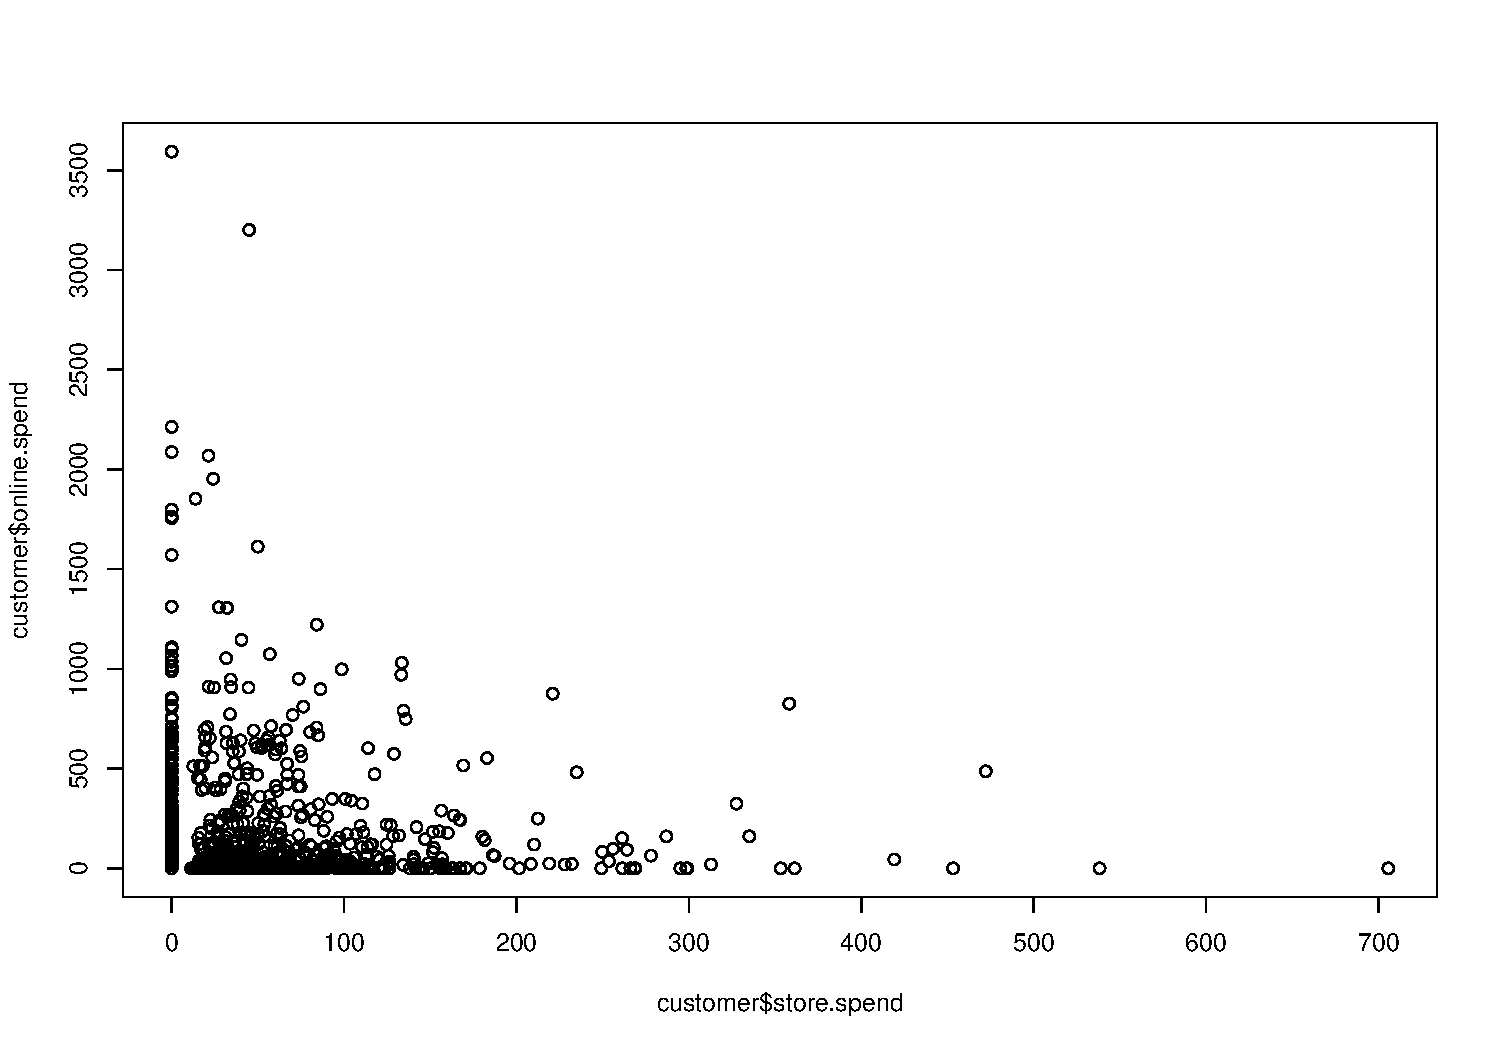
\includegraphics[width=0.5\textwidth,height=\textheight]{004_relationships_between_continuous_variables_files/figure-beamer/unnamed-chunk-6-1.pdf}
\end{center}
\end{frame}

\begin{frame}[fragile]{}
\phantomsection\label{section-9}
\begin{itemize}
\tightlist
\item
  \textbf{Scatterplots: the base R way}
\end{itemize}

\tiny

\begin{Shaded}
\begin{Highlighting}[]
\FunctionTok{plot}\NormalTok{(}\AttributeTok{x =}\NormalTok{ customer}\SpecialCharTok{$}\NormalTok{store.spend, }\AttributeTok{y =}\NormalTok{ customer}\SpecialCharTok{$}\NormalTok{online.spend,}
     \AttributeTok{cex=}\FloatTok{0.7}\NormalTok{,}
     \AttributeTok{main=}\StringTok{"Customers as of June 2014"}\NormalTok{, }
     \AttributeTok{xlab=}\StringTok{"Prior 12 months in{-}store sales ($)"}\NormalTok{, }
     \AttributeTok{ylab=}\StringTok{"Prior 12 months online sales ($)"}\NormalTok{)}
\end{Highlighting}
\end{Shaded}

\begin{center}
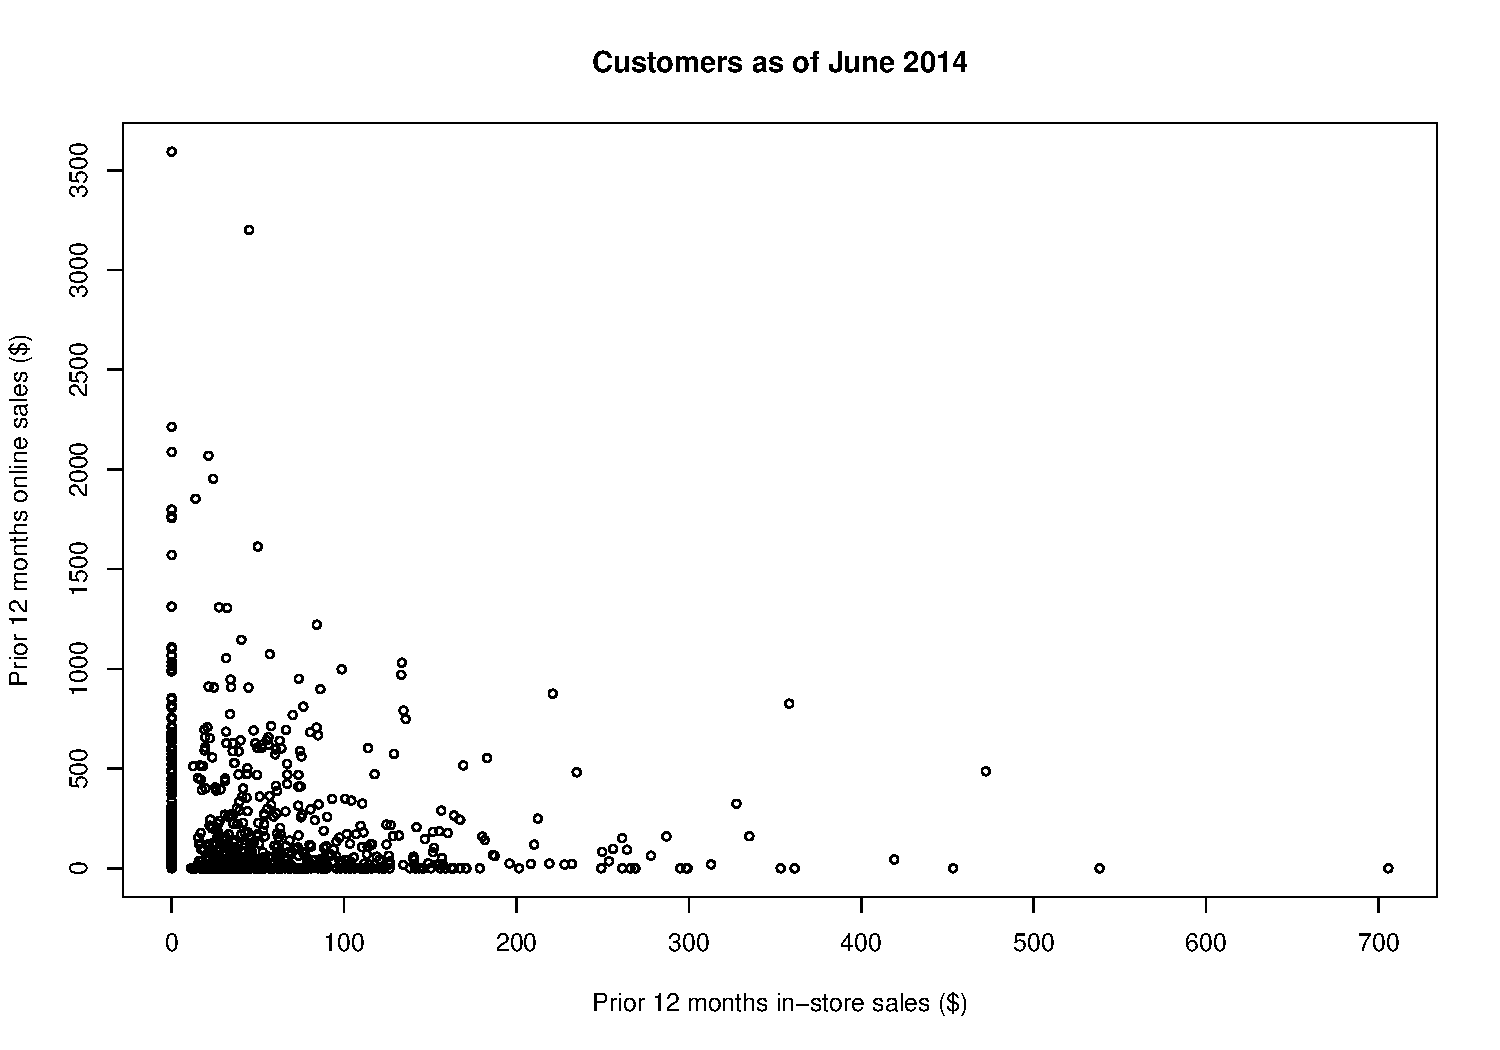
\includegraphics[width=0.5\textwidth,height=\textheight]{004_relationships_between_continuous_variables_files/figure-beamer/unnamed-chunk-7-1.pdf}
\end{center}
\end{frame}

\begin{frame}[fragile]{}
\phantomsection\label{section-10}
\begin{itemize}
\tightlist
\item
  \textbf{Scatterplots: the base R way}
\end{itemize}

\tiny

\begin{Shaded}
\begin{Highlighting}[]
\NormalTok{my.col }\OtherTok{\textless{}{-}} \FunctionTok{c}\NormalTok{(}\StringTok{"black"}\NormalTok{, }\StringTok{"green3"}\NormalTok{)}
\NormalTok{my.pch }\OtherTok{\textless{}{-}} \FunctionTok{c}\NormalTok{(}\DecValTok{1}\NormalTok{, }\DecValTok{19}\NormalTok{)}
\FunctionTok{plot}\NormalTok{(}\AttributeTok{x =}\NormalTok{ customer}\SpecialCharTok{$}\NormalTok{store.spend, }\AttributeTok{y =}\NormalTok{ customer}\SpecialCharTok{$}\NormalTok{online.spend,}
     \AttributeTok{cex=}\FloatTok{0.7}\NormalTok{, }\AttributeTok{col=}\NormalTok{my.col[customer}\SpecialCharTok{$}\NormalTok{email], }\AttributeTok{pch=}\NormalTok{my.pch[customer}\SpecialCharTok{$}\NormalTok{email],}
     \AttributeTok{main=}\StringTok{"Customers as of June 2014"}\NormalTok{, }
     \AttributeTok{xlab=}\StringTok{"Prior 12 months in{-}store sales ($)"}\NormalTok{, }
     \AttributeTok{ylab=}\StringTok{"Prior 12 months online sales ($)"}\NormalTok{)}
\end{Highlighting}
\end{Shaded}

\begin{center}
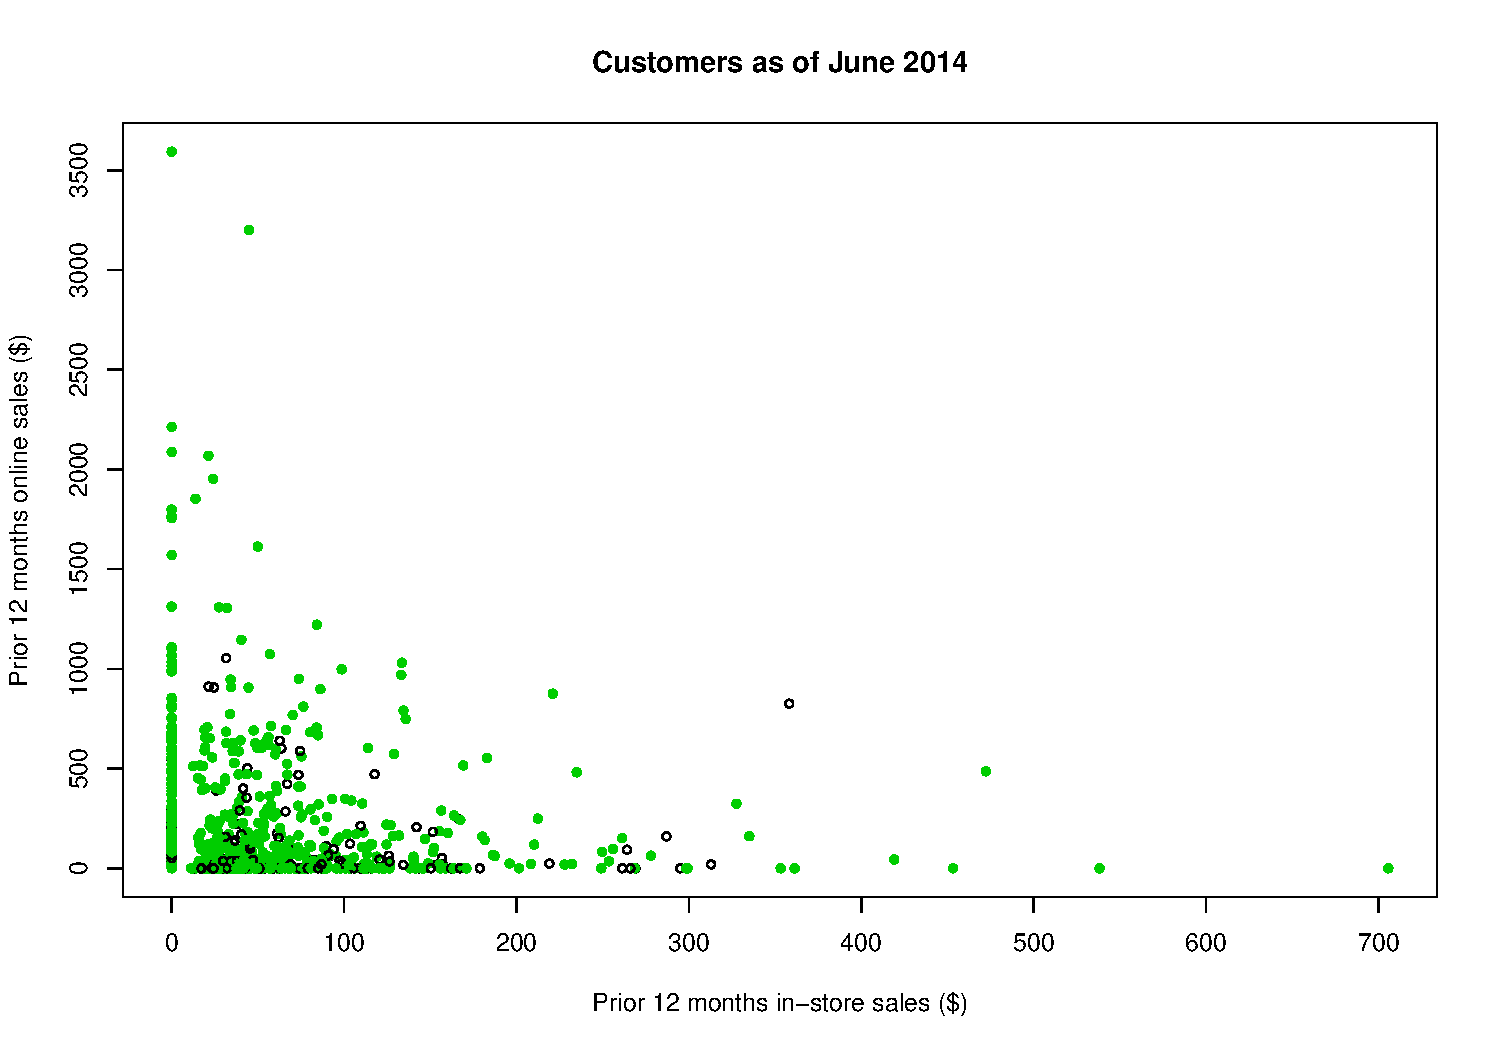
\includegraphics[width=0.5\textwidth,height=\textheight]{004_relationships_between_continuous_variables_files/figure-beamer/unnamed-chunk-8-1.pdf}
\end{center}
\end{frame}

\begin{frame}[fragile]{}
\phantomsection\label{section-11}
\begin{itemize}
\tightlist
\item
  \textbf{Scatterplots: the base R way}
\end{itemize}

\tiny

\begin{Shaded}
\begin{Highlighting}[]
\NormalTok{my.col }\OtherTok{\textless{}{-}} \FunctionTok{c}\NormalTok{(}\StringTok{"black"}\NormalTok{, }\StringTok{"green3"}\NormalTok{)}
\NormalTok{my.pch }\OtherTok{\textless{}{-}} \FunctionTok{c}\NormalTok{(}\DecValTok{1}\NormalTok{, }\DecValTok{19}\NormalTok{)}
\FunctionTok{plot}\NormalTok{(}\AttributeTok{x =}\NormalTok{ customer}\SpecialCharTok{$}\NormalTok{store.spend, }\AttributeTok{y =}\NormalTok{ customer}\SpecialCharTok{$}\NormalTok{online.spend,}
     \AttributeTok{cex=}\FloatTok{0.7}\NormalTok{, }\AttributeTok{col=}\NormalTok{my.col[customer}\SpecialCharTok{$}\NormalTok{email], }\AttributeTok{pch=}\NormalTok{my.pch[customer}\SpecialCharTok{$}\NormalTok{email],}
     \AttributeTok{main=}\StringTok{"Customers as of June 2014"}\NormalTok{, }
     \AttributeTok{xlab=}\StringTok{"Prior 12 months in{-}store sales ($)"}\NormalTok{, }
     \AttributeTok{ylab=}\StringTok{"Prior 12 months online sales ($)"}\NormalTok{)}
\FunctionTok{legend}\NormalTok{(}\AttributeTok{x=}\StringTok{"topright"}\NormalTok{, }\AttributeTok{legend=}\FunctionTok{paste}\NormalTok{(}\StringTok{"email on file:"}\NormalTok{, }\FunctionTok{levels}\NormalTok{(customer}\SpecialCharTok{$}\NormalTok{email)), }\AttributeTok{col=}\NormalTok{my.col, }\AttributeTok{pch=}\NormalTok{my.pch)}
\end{Highlighting}
\end{Shaded}

\begin{center}
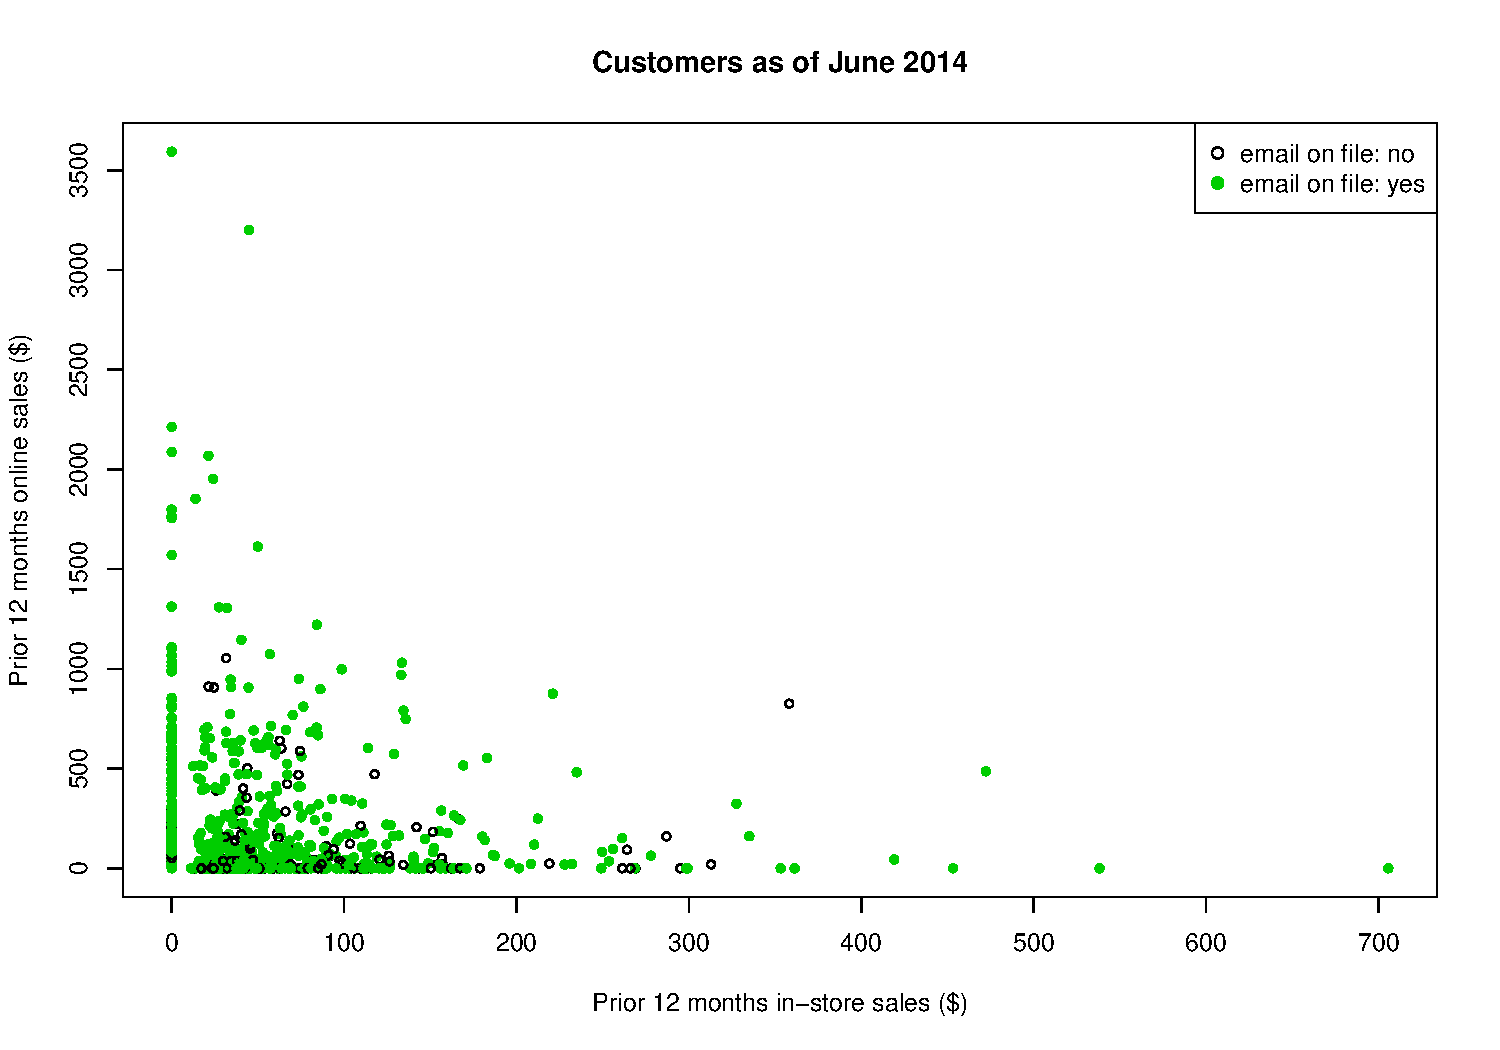
\includegraphics[width=0.5\textwidth,height=\textheight]{004_relationships_between_continuous_variables_files/figure-beamer/unnamed-chunk-9-1.pdf}
\end{center}
\end{frame}

\begin{frame}[fragile]{}
\phantomsection\label{section-12}
\begin{itemize}
\tightlist
\item
  \textbf{Scatterplots: the base R way}
\end{itemize}

\tiny

\begin{Shaded}
\begin{Highlighting}[]
\NormalTok{my.col }\OtherTok{\textless{}{-}} \FunctionTok{c}\NormalTok{(}\StringTok{"black"}\NormalTok{, }\StringTok{"green3"}\NormalTok{)}
\NormalTok{my.pch }\OtherTok{\textless{}{-}} \FunctionTok{c}\NormalTok{(}\DecValTok{1}\NormalTok{, }\DecValTok{19}\NormalTok{)}
\FunctionTok{plot}\NormalTok{(}\AttributeTok{x =}\NormalTok{ customer}\SpecialCharTok{$}\NormalTok{store.spend }\SpecialCharTok{+} \DecValTok{1}\NormalTok{, }\AttributeTok{y =}\NormalTok{ customer}\SpecialCharTok{$}\NormalTok{online.spend }\SpecialCharTok{+} \DecValTok{1}\NormalTok{,}
     \AttributeTok{cex=}\FloatTok{0.7}\NormalTok{, }\AttributeTok{col=}\NormalTok{my.col[customer}\SpecialCharTok{$}\NormalTok{email], }\AttributeTok{pch=}\NormalTok{my.pch[customer}\SpecialCharTok{$}\NormalTok{email],}
     \AttributeTok{log =}\StringTok{"xy"}\NormalTok{,}
     \AttributeTok{main=}\StringTok{"Customers as of June 2014"}\NormalTok{, }
     \AttributeTok{xlab=}\StringTok{"Prior 12 months in{-}store sales ($)"}\NormalTok{, }
     \AttributeTok{ylab=}\StringTok{"Prior 12 months online sales ($)"}\NormalTok{)}
\FunctionTok{legend}\NormalTok{(}\AttributeTok{x=}\StringTok{"topright"}\NormalTok{, }\AttributeTok{legend=}\FunctionTok{paste}\NormalTok{(}\StringTok{"email on file:"}\NormalTok{, }\FunctionTok{levels}\NormalTok{(customer}\SpecialCharTok{$}\NormalTok{email)), }\AttributeTok{col=}\NormalTok{my.col, }\AttributeTok{pch=}\NormalTok{my.pch)}
\end{Highlighting}
\end{Shaded}

\begin{center}
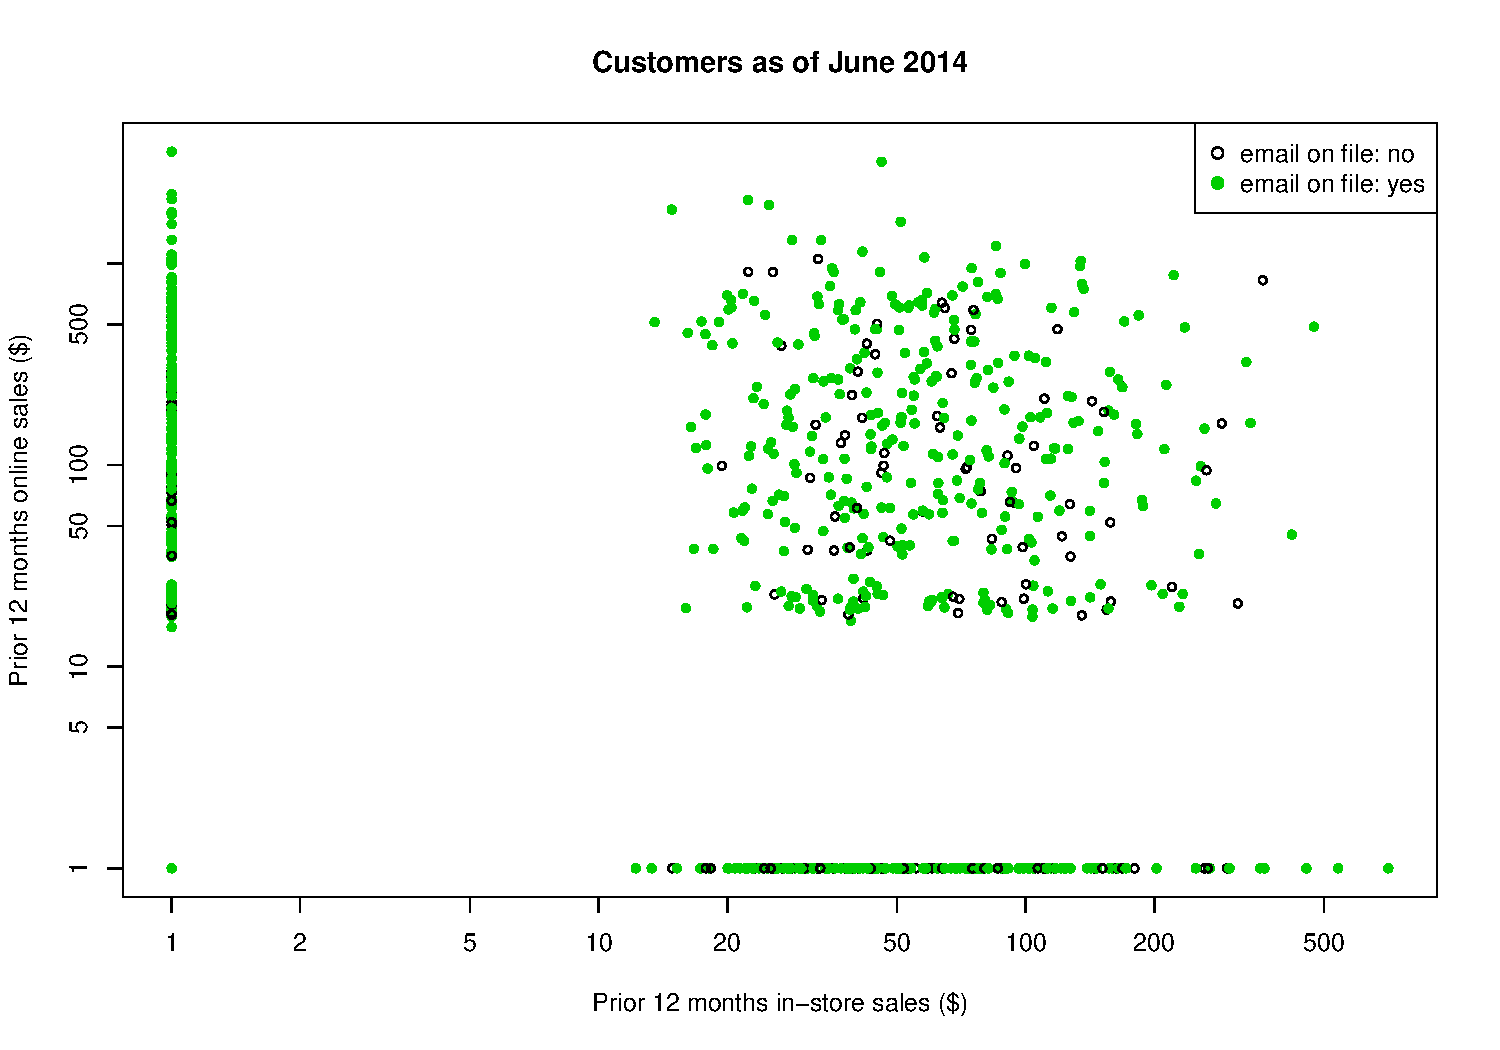
\includegraphics[width=0.5\textwidth,height=\textheight]{004_relationships_between_continuous_variables_files/figure-beamer/unnamed-chunk-10-1.pdf}
\end{center}
\end{frame}

\begin{frame}[fragile]{}
\phantomsection\label{section-13}
\begin{itemize}
\tightlist
\item
  \textbf{Scatterplots: the tidyverse way}
\end{itemize}

\tiny

\begin{Shaded}
\begin{Highlighting}[]
\NormalTok{customer }\SpecialCharTok{|\textgreater{}} \FunctionTok{ggplot}\NormalTok{() }\SpecialCharTok{+}
  \FunctionTok{geom\_point}\NormalTok{(}\FunctionTok{aes}\NormalTok{(}\AttributeTok{x =}\NormalTok{ store.spend, }\AttributeTok{y =}\NormalTok{ online.spend, }\AttributeTok{color =}\NormalTok{ email))}
\end{Highlighting}
\end{Shaded}

\begin{center}
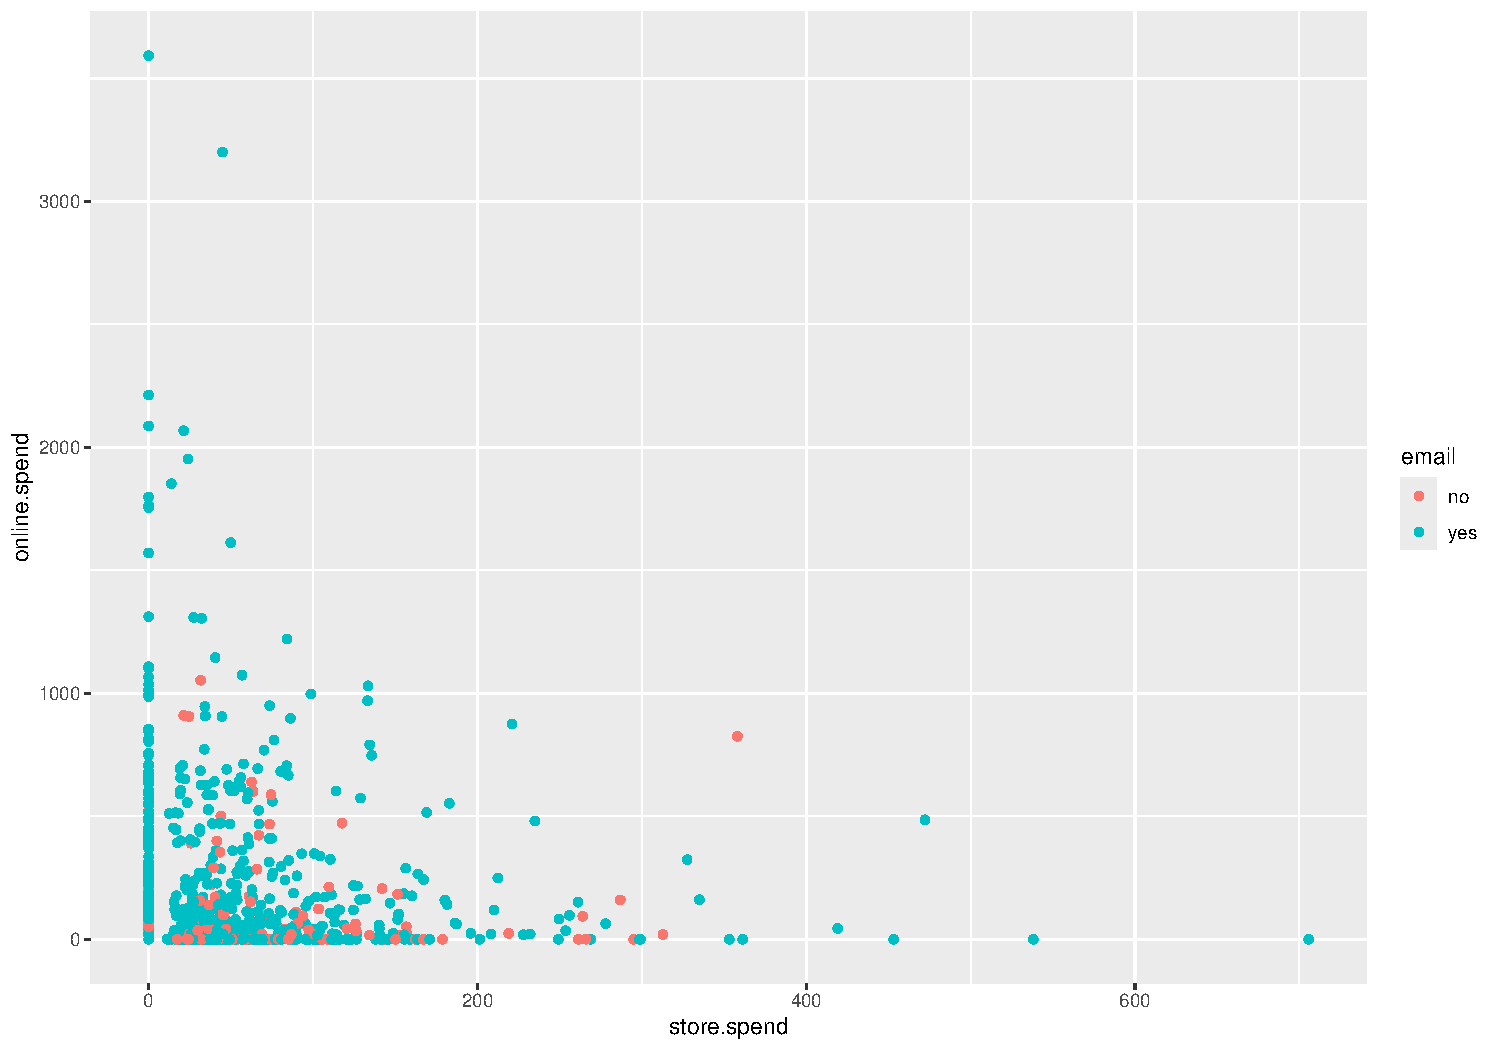
\includegraphics[width=0.5\textwidth,height=\textheight]{004_relationships_between_continuous_variables_files/figure-beamer/unnamed-chunk-11-1.pdf}
\end{center}
\end{frame}

\begin{frame}[fragile]{}
\phantomsection\label{section-14}
\begin{itemize}
\tightlist
\item
  \textbf{Scatterplots: the tidyverse way}
\end{itemize}

\tiny

\begin{Shaded}
\begin{Highlighting}[]
\NormalTok{customer }\SpecialCharTok{|\textgreater{}} \FunctionTok{ggplot}\NormalTok{() }\SpecialCharTok{+}
  \FunctionTok{geom\_point}\NormalTok{(}\FunctionTok{aes}\NormalTok{(}\AttributeTok{x =}\NormalTok{ store.spend, }\AttributeTok{y =}\NormalTok{ online.spend, }\AttributeTok{color =}\NormalTok{ email, }\AttributeTok{shape =}\NormalTok{ email)) }\SpecialCharTok{+}
  \FunctionTok{scale\_color\_manual}\NormalTok{(}\AttributeTok{values =} \FunctionTok{c}\NormalTok{(}\StringTok{"black"}\NormalTok{, }\StringTok{"green3"}\NormalTok{), }\AttributeTok{labels =} \FunctionTok{c}\NormalTok{(}\StringTok{"email on file: no"}\NormalTok{, }\StringTok{"email on file: yes"}\NormalTok{)) }\SpecialCharTok{+}
  \FunctionTok{scale\_shape\_manual}\NormalTok{(}\AttributeTok{values =} \FunctionTok{c}\NormalTok{(}\DecValTok{1}\NormalTok{, }\DecValTok{19}\NormalTok{), }\AttributeTok{labels =} \FunctionTok{c}\NormalTok{(}\StringTok{"email on file: no"}\NormalTok{, }\StringTok{"email on file: yes"}\NormalTok{))}
\end{Highlighting}
\end{Shaded}

\begin{center}
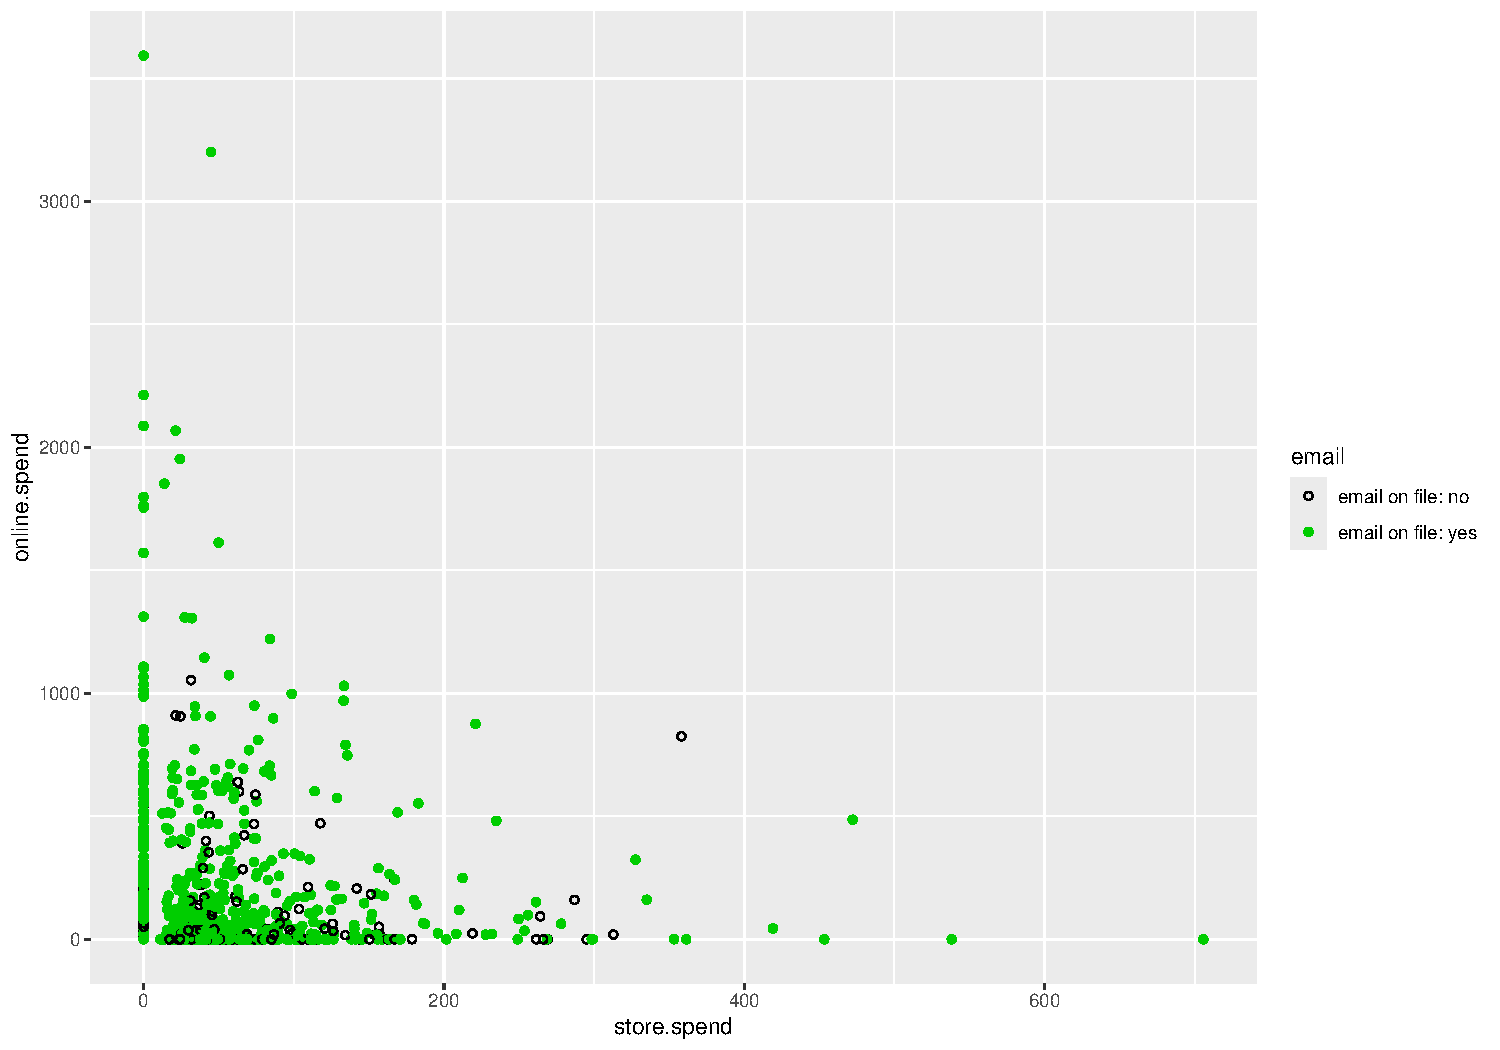
\includegraphics[width=0.5\textwidth,height=\textheight]{004_relationships_between_continuous_variables_files/figure-beamer/unnamed-chunk-12-1.pdf}
\end{center}
\end{frame}

\begin{frame}[fragile]{}
\phantomsection\label{section-15}
\begin{itemize}
\tightlist
\item
  \textbf{Scatterplots: the tidyverse way}
\end{itemize}

\tiny

\begin{Shaded}
\begin{Highlighting}[]
\NormalTok{customer }\SpecialCharTok{|\textgreater{}} \FunctionTok{ggplot}\NormalTok{() }\SpecialCharTok{+}
  \FunctionTok{geom\_point}\NormalTok{(}\FunctionTok{aes}\NormalTok{(}\AttributeTok{x =}\NormalTok{ store.spend, }\AttributeTok{y =}\NormalTok{ online.spend, }\AttributeTok{color =}\NormalTok{ email, }\AttributeTok{shape =}\NormalTok{ email)) }\SpecialCharTok{+}
  \FunctionTok{scale\_color\_manual}\NormalTok{(}\AttributeTok{values =} \FunctionTok{c}\NormalTok{(}\StringTok{"black"}\NormalTok{, }\StringTok{"green3"}\NormalTok{), }\AttributeTok{labels =} \FunctionTok{c}\NormalTok{(}\StringTok{"email on file: no"}\NormalTok{, }\StringTok{"email on file: yes"}\NormalTok{)) }\SpecialCharTok{+}
  \FunctionTok{scale\_shape\_manual}\NormalTok{(}\AttributeTok{values =} \FunctionTok{c}\NormalTok{(}\DecValTok{1}\NormalTok{, }\DecValTok{19}\NormalTok{), }\AttributeTok{labels =} \FunctionTok{c}\NormalTok{(}\StringTok{"email on file: no"}\NormalTok{, }\StringTok{"email on file: yes"}\NormalTok{)) }\SpecialCharTok{+}
  \FunctionTok{scale\_x\_continuous}\NormalTok{(}\AttributeTok{trans =} \StringTok{"log1p"}\NormalTok{, }\AttributeTok{breaks =} \FunctionTok{c}\NormalTok{(}\DecValTok{1}\NormalTok{, }\DecValTok{2}\NormalTok{, }\DecValTok{5}\NormalTok{, }\DecValTok{10}\NormalTok{, }\DecValTok{20}\NormalTok{, }\DecValTok{50}\NormalTok{, }\DecValTok{100}\NormalTok{, }\DecValTok{500}\NormalTok{)) }\SpecialCharTok{+} 
  \FunctionTok{scale\_y\_continuous}\NormalTok{(}\AttributeTok{trans =} \StringTok{"log1p"}\NormalTok{, }\AttributeTok{breaks =} \FunctionTok{c}\NormalTok{(}\DecValTok{1}\NormalTok{, }\DecValTok{5}\NormalTok{, }\DecValTok{50}\NormalTok{, }\DecValTok{500}\NormalTok{))}
\end{Highlighting}
\end{Shaded}

\begin{center}
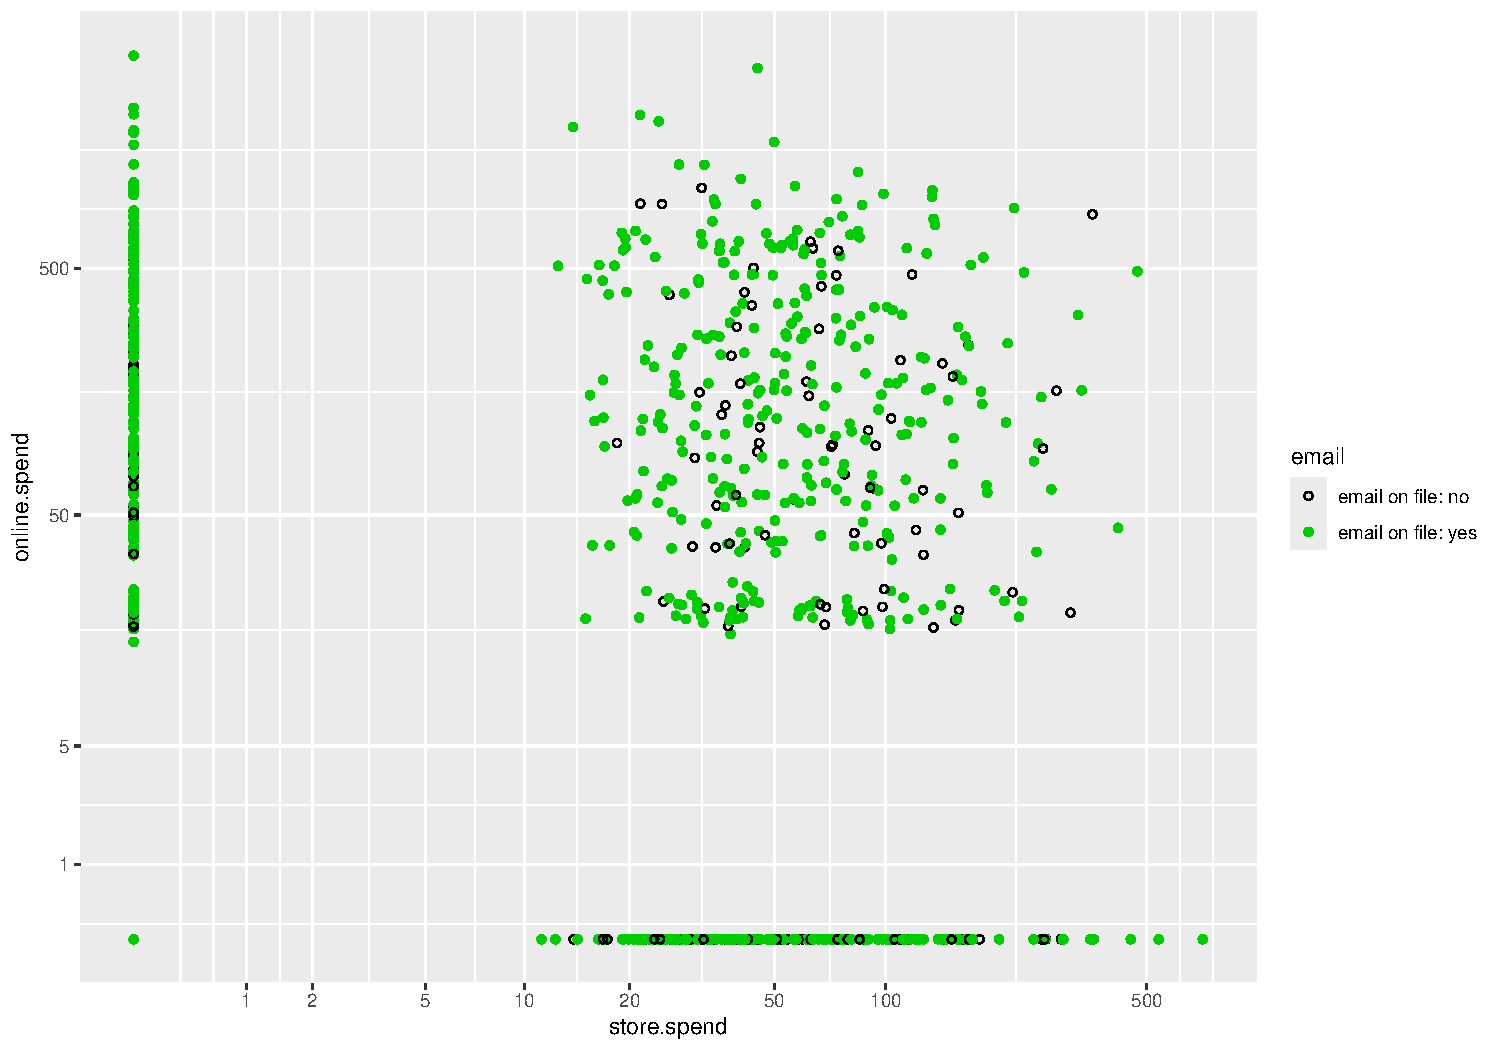
\includegraphics[width=0.5\textwidth,height=\textheight]{004_relationships_between_continuous_variables_files/figure-beamer/unnamed-chunk-13-1.pdf}
\end{center}
\end{frame}

\begin{frame}[fragile]{}
\phantomsection\label{section-16}
\begin{itemize}
\tightlist
\item
  \textbf{Scatterplots: the tidyverse way}
\end{itemize}

\tiny

\begin{Shaded}
\begin{Highlighting}[]
\NormalTok{customer }\SpecialCharTok{|\textgreater{}} \FunctionTok{ggplot}\NormalTok{() }\SpecialCharTok{+}
  \FunctionTok{geom\_point}\NormalTok{(}\FunctionTok{aes}\NormalTok{(}\AttributeTok{x =}\NormalTok{ store.spend, }\AttributeTok{y =}\NormalTok{ online.spend, }\AttributeTok{color =}\NormalTok{ email, }\AttributeTok{shape =}\NormalTok{ email)) }\SpecialCharTok{+}
  \FunctionTok{scale\_color\_manual}\NormalTok{(}\AttributeTok{values =} \FunctionTok{c}\NormalTok{(}\StringTok{"black"}\NormalTok{, }\StringTok{"green3"}\NormalTok{), }\AttributeTok{labels =} \FunctionTok{c}\NormalTok{(}\StringTok{"email on file: no"}\NormalTok{, }\StringTok{"email on file: yes"}\NormalTok{)) }\SpecialCharTok{+}
  \FunctionTok{scale\_shape\_manual}\NormalTok{(}\AttributeTok{values =} \FunctionTok{c}\NormalTok{(}\DecValTok{1}\NormalTok{, }\DecValTok{19}\NormalTok{), }\AttributeTok{labels =} \FunctionTok{c}\NormalTok{(}\StringTok{"email on file: no"}\NormalTok{, }\StringTok{"email on file: yes"}\NormalTok{)) }\SpecialCharTok{+}
  \FunctionTok{scale\_x\_continuous}\NormalTok{(}\AttributeTok{trans =} \StringTok{"log1p"}\NormalTok{, }\AttributeTok{breaks =} \FunctionTok{c}\NormalTok{(}\DecValTok{1}\NormalTok{, }\DecValTok{2}\NormalTok{, }\DecValTok{5}\NormalTok{, }\DecValTok{10}\NormalTok{, }\DecValTok{20}\NormalTok{, }\DecValTok{50}\NormalTok{, }\DecValTok{100}\NormalTok{, }\DecValTok{500}\NormalTok{)) }\SpecialCharTok{+} 
  \FunctionTok{scale\_y\_continuous}\NormalTok{(}\AttributeTok{trans =} \StringTok{"log1p"}\NormalTok{, }\AttributeTok{breaks =} \FunctionTok{c}\NormalTok{(}\DecValTok{1}\NormalTok{, }\DecValTok{5}\NormalTok{, }\DecValTok{50}\NormalTok{, }\DecValTok{500}\NormalTok{)) }\SpecialCharTok{+}
  \FunctionTok{labs}\NormalTok{(}\AttributeTok{x =} \StringTok{"Prior 12 months in{-}store sales ($)"}\NormalTok{, }\AttributeTok{y =} \StringTok{"Prior 12 months online sales ($)"}\NormalTok{,}
       \AttributeTok{title =} \StringTok{"Customers as of June 2014"}\NormalTok{)}
\end{Highlighting}
\end{Shaded}

\begin{center}
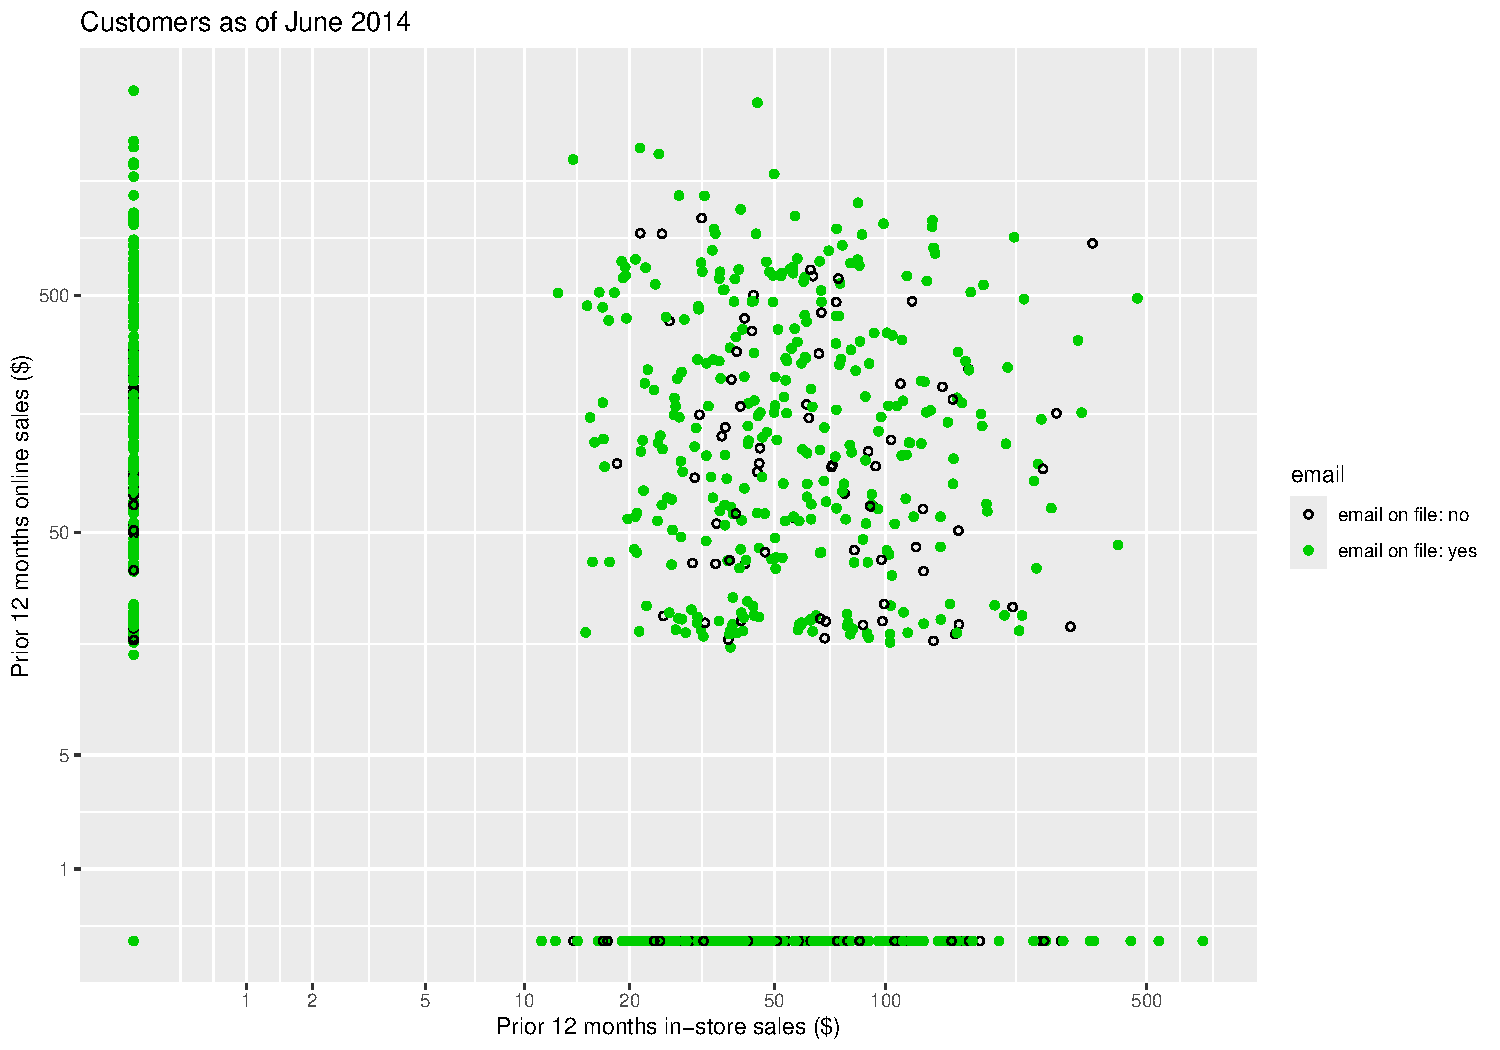
\includegraphics[width=0.5\textwidth,height=\textheight]{004_relationships_between_continuous_variables_files/figure-beamer/unnamed-chunk-14-1.pdf}
\end{center}
\end{frame}

\begin{frame}{}
\phantomsection\label{section-17}
\begin{itemize}
\item
  \textbf{Correlation Coefficients}

  \begin{itemize}
  \tightlist
  \item
    Pearson correlation coefficient for a sample
  \end{itemize}
\end{itemize}

\small

\[r_{xy} = \frac{\sum_{i=1}^n (x_i - \bar{x})(y_i - \bar{y})}{\sqrt{\sum_{i=1}^n (x_i - \bar{x})^2}\sqrt{\sum_{i=1}^n (y_i - \bar{y})^2}}\]
Where \(n\) is the sample size, we must have paired numeric data
\(\{ (x_1, y_1), ..., (x_n, y_n) \}\), \(\bar{x} = \sum_{i=1}^n x_i\)
and \(\bar{y} = \sum_{i=1}^n y_i\)

\begin{itemize}
\tightlist
\item
  This is a ``nasty'' formula but we can brake it down in smaller chunks
\end{itemize}
\end{frame}

\begin{frame}[fragile]{}
\phantomsection\label{section-18}
\begin{itemize}
\item
  \textbf{Correlation Coefficients}

  \begin{itemize}
  \tightlist
  \item
    Pearson correlation coefficient for a sample
  \end{itemize}
\end{itemize}

\tiny

\begin{Shaded}
\begin{Highlighting}[]
\NormalTok{age\_mean }\OtherTok{\textless{}{-}} \FunctionTok{mean}\NormalTok{(customer}\SpecialCharTok{$}\NormalTok{age)}
\NormalTok{age\_credit.score }\OtherTok{\textless{}{-}} \FunctionTok{mean}\NormalTok{(customer}\SpecialCharTok{$}\NormalTok{credit.score)}
\NormalTok{numerator }\OtherTok{\textless{}{-}} \FunctionTok{sum}\NormalTok{((customer}\SpecialCharTok{$}\NormalTok{age }\SpecialCharTok{{-}}\NormalTok{ age\_mean) }\SpecialCharTok{*}\NormalTok{ (customer}\SpecialCharTok{$}\NormalTok{credit.score }\SpecialCharTok{{-}}\NormalTok{ age\_credit.score)) }
\NormalTok{denominator }\OtherTok{\textless{}{-}} \FunctionTok{sqrt}\NormalTok{(}\FunctionTok{sum}\NormalTok{((customer}\SpecialCharTok{$}\NormalTok{age }\SpecialCharTok{{-}}\NormalTok{ age\_mean)}\SpecialCharTok{\^{}}\DecValTok{2}\NormalTok{)) }\SpecialCharTok{*} \FunctionTok{sqrt}\NormalTok{(}\FunctionTok{sum}\NormalTok{(((customer}\SpecialCharTok{$}\NormalTok{credit.score }\SpecialCharTok{{-}}\NormalTok{ age\_credit.score)}\SpecialCharTok{\^{}}\DecValTok{2}\NormalTok{)))}
\NormalTok{pearson\_corr }\OtherTok{\textless{}{-}}\NormalTok{ numerator }\SpecialCharTok{/}\NormalTok{ denominator}
\NormalTok{pearson\_corr}
\end{Highlighting}
\end{Shaded}

\begin{verbatim}
[1] 0.2545045
\end{verbatim}

\small

\begin{itemize}
\tightlist
\item
  \textbf{But don't worry be happy!!!: Use \texttt{cor}}
\end{itemize}

\tiny

\begin{Shaded}
\begin{Highlighting}[]
\FunctionTok{cor}\NormalTok{(customer}\SpecialCharTok{$}\NormalTok{age, customer}\SpecialCharTok{$}\NormalTok{credit.score, }\AttributeTok{method =} \StringTok{\textquotesingle{}pearson\textquotesingle{}}\NormalTok{)}
\end{Highlighting}
\end{Shaded}

\begin{verbatim}
[1] 0.2545045
\end{verbatim}
\end{frame}

\begin{frame}[fragile]{}
\phantomsection\label{section-19}
\begin{itemize}
\item
  \textbf{Correlation matrices}

  \begin{itemize}
  \tightlist
  \item
    Pearson correlation coefficients for samples in a tibble
  \end{itemize}
\end{itemize}

\tiny

\begin{Shaded}
\begin{Highlighting}[]
\FunctionTok{library}\NormalTok{(corrr) }\CommentTok{\# Remember to install the package if it is not installed}
\NormalTok{correlation\_matrix }\OtherTok{\textless{}{-}}\NormalTok{ customer }\SpecialCharTok{|\textgreater{}} 
  \FunctionTok{select}\NormalTok{(}\FunctionTok{where}\NormalTok{(is.numeric)) }\SpecialCharTok{|\textgreater{}} 
  \FunctionTok{correlate}\NormalTok{(}\AttributeTok{use =} \StringTok{"pairwise.complete.obs"}\NormalTok{, }\CommentTok{\# There are NA values}
            \AttributeTok{method =} \StringTok{"pearson"}\NormalTok{,}
            \AttributeTok{diagonal =} \ConstantTok{NA}\NormalTok{)}
\NormalTok{correlation\_matrix }\CommentTok{\# Ups!!! The tibble is wide. Check out the tibble in your console}
\end{Highlighting}
\end{Shaded}

\begin{verbatim}
# A tibble: 8 x 9
  term             age credit.score distance.to.store online.visits online.trans
  <chr>          <dbl>        <dbl>             <dbl>         <dbl>        <dbl>
1 age         NA            0.255             0.00199       -0.0614     -0.0630 
2 credit.sco~  0.255       NA                -0.0233        -0.0108     -0.00502
3 distance.t~  0.00199     -0.0233           NA             -0.0146     -0.0196 
4 online.vis~ -0.0614      -0.0108           -0.0146        NA           0.987  
5 online.tra~ -0.0630      -0.00502          -0.0196         0.987      NA      
6 online.spe~ -0.0607      -0.00608          -0.0204         0.982       0.993  
7 store.trans  0.0242       0.0404           -0.277         -0.0367     -0.0402 
8 store.spend  0.00384      0.0423           -0.241         -0.0507     -0.0522 
# i 3 more variables: online.spend <dbl>, store.trans <dbl>, store.spend <dbl>
\end{verbatim}
\end{frame}

\begin{frame}[fragile]{}
\phantomsection\label{section-20}
\begin{itemize}
\item
  \textbf{Correlation matrices}

  \begin{itemize}
  \tightlist
  \item
    Pearson correlation coefficients for samples in a tibble
  \end{itemize}
\end{itemize}

\tiny

\begin{Shaded}
\begin{Highlighting}[]
\NormalTok{correlation\_matrix }\SpecialCharTok{|\textgreater{}} \FunctionTok{autoplot}\NormalTok{(}\AttributeTok{triangular =} \StringTok{"lower"}\NormalTok{)}
\end{Highlighting}
\end{Shaded}

\begin{center}
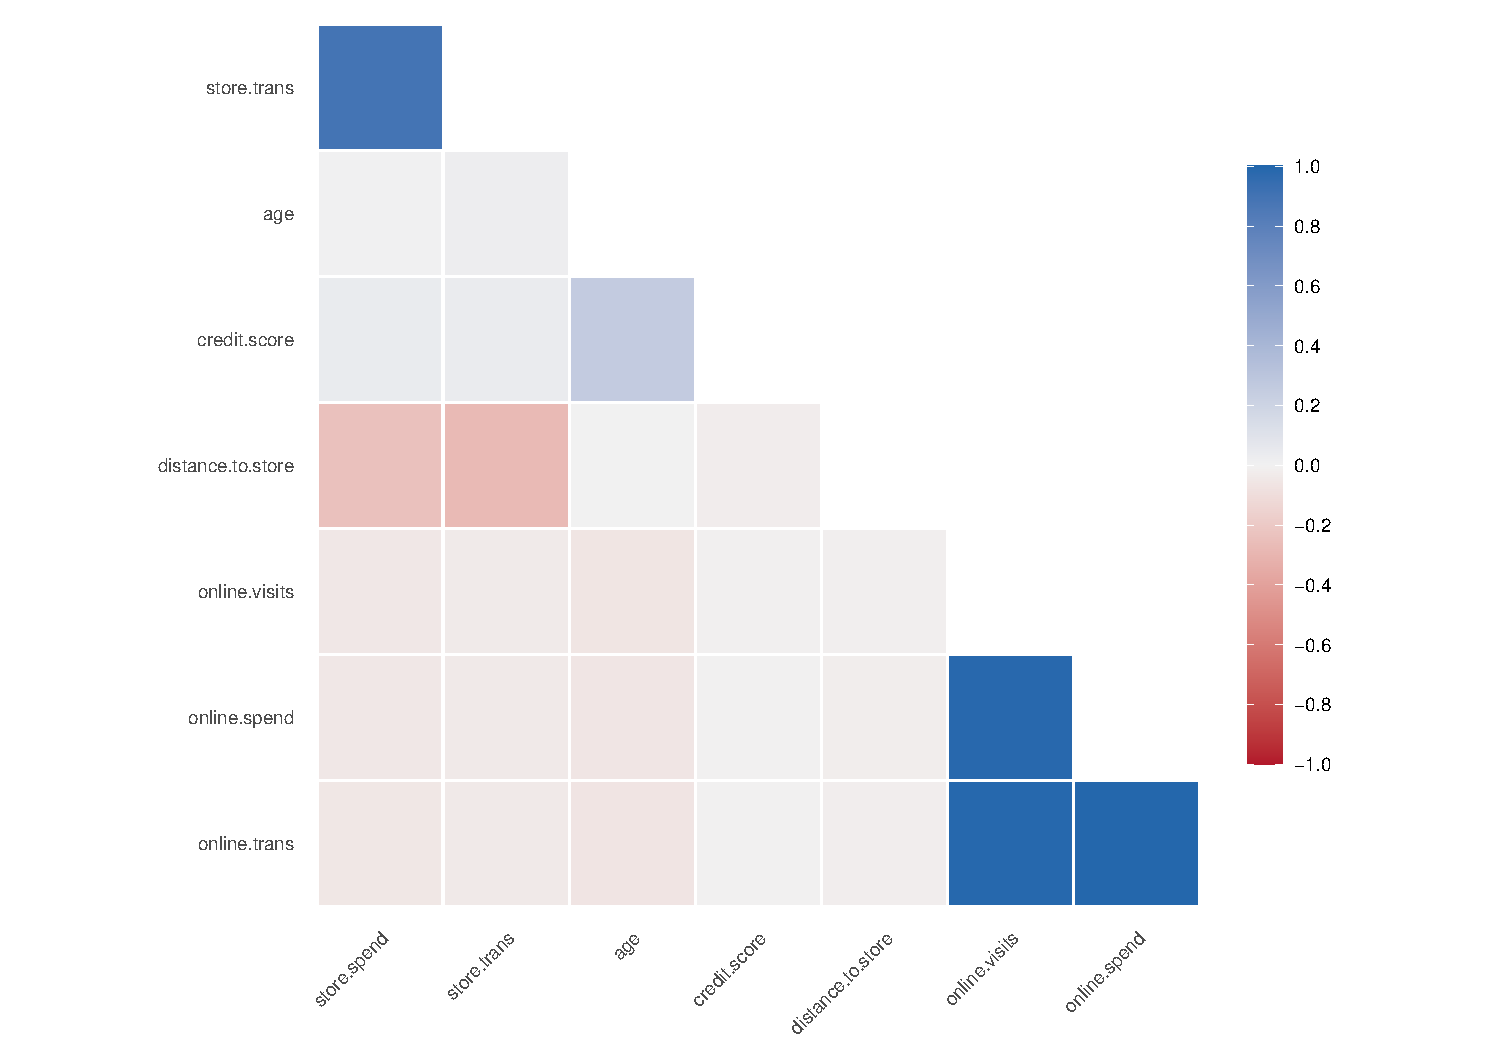
\includegraphics[width=0.5\textwidth,height=\textheight]{004_relationships_between_continuous_variables_files/figure-beamer/unnamed-chunk-18-1.pdf}
\end{center}
\end{frame}

\begin{frame}[fragile]{}
\phantomsection\label{section-21}
\begin{itemize}
\tightlist
\item
  \textbf{Transforming variables}
\end{itemize}

\tiny

\begin{Shaded}
\begin{Highlighting}[]
\FunctionTok{cor}\NormalTok{(customer}\SpecialCharTok{$}\NormalTok{store.spend, customer}\SpecialCharTok{$}\NormalTok{distance.to.store)}
\end{Highlighting}
\end{Shaded}

\begin{verbatim}
[1] -0.2414949
\end{verbatim}

\begin{Shaded}
\begin{Highlighting}[]
\NormalTok{customer }\SpecialCharTok{|\textgreater{}} \FunctionTok{ggplot}\NormalTok{() }\SpecialCharTok{+}
  \FunctionTok{geom\_point}\NormalTok{(}\FunctionTok{aes}\NormalTok{(}\AttributeTok{x =}\NormalTok{ distance.to.store, }\AttributeTok{y =}\NormalTok{ store.spend))}
\end{Highlighting}
\end{Shaded}

\begin{center}
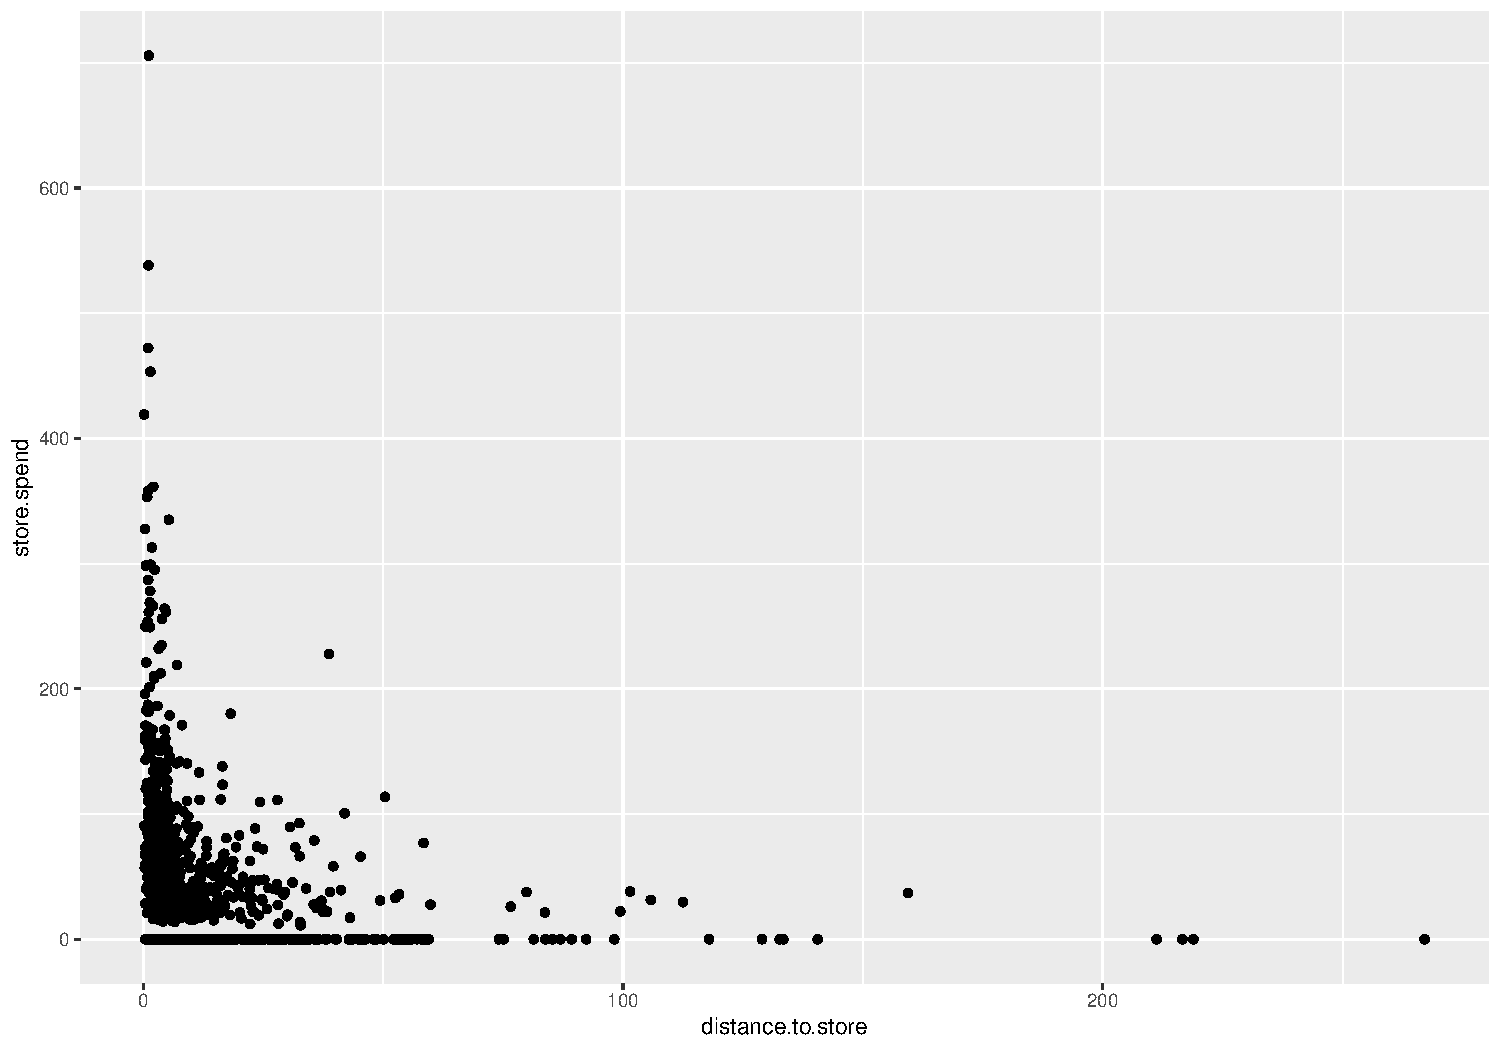
\includegraphics[width=0.5\textwidth,height=\textheight]{004_relationships_between_continuous_variables_files/figure-beamer/unnamed-chunk-20-1.pdf}
\end{center}
\end{frame}

\begin{frame}[fragile]{}
\phantomsection\label{section-22}
\begin{itemize}
\tightlist
\item
  \textbf{Transforming variables}
\end{itemize}

\tiny

\begin{Shaded}
\begin{Highlighting}[]
\FunctionTok{cor}\NormalTok{(customer}\SpecialCharTok{$}\NormalTok{store.spend, }\DecValTok{1} \SpecialCharTok{/} \FunctionTok{sqrt}\NormalTok{(customer}\SpecialCharTok{$}\NormalTok{distance.to.store))}
\end{Highlighting}
\end{Shaded}

\begin{verbatim}
[1] 0.4843334
\end{verbatim}

\begin{Shaded}
\begin{Highlighting}[]
\NormalTok{customer }\SpecialCharTok{|\textgreater{}}
  \FunctionTok{mutate}\NormalTok{(}\AttributeTok{distance.to.store\_trans =} \DecValTok{1} \SpecialCharTok{/} \FunctionTok{sqrt}\NormalTok{(distance.to.store)) }\SpecialCharTok{|\textgreater{}}
  \FunctionTok{ggplot}\NormalTok{() }\SpecialCharTok{+}
  \FunctionTok{geom\_point}\NormalTok{(}\FunctionTok{aes}\NormalTok{(}\AttributeTok{x =}\NormalTok{ distance.to.store\_trans, }\AttributeTok{y =}\NormalTok{ store.spend))}
\end{Highlighting}
\end{Shaded}

\begin{center}
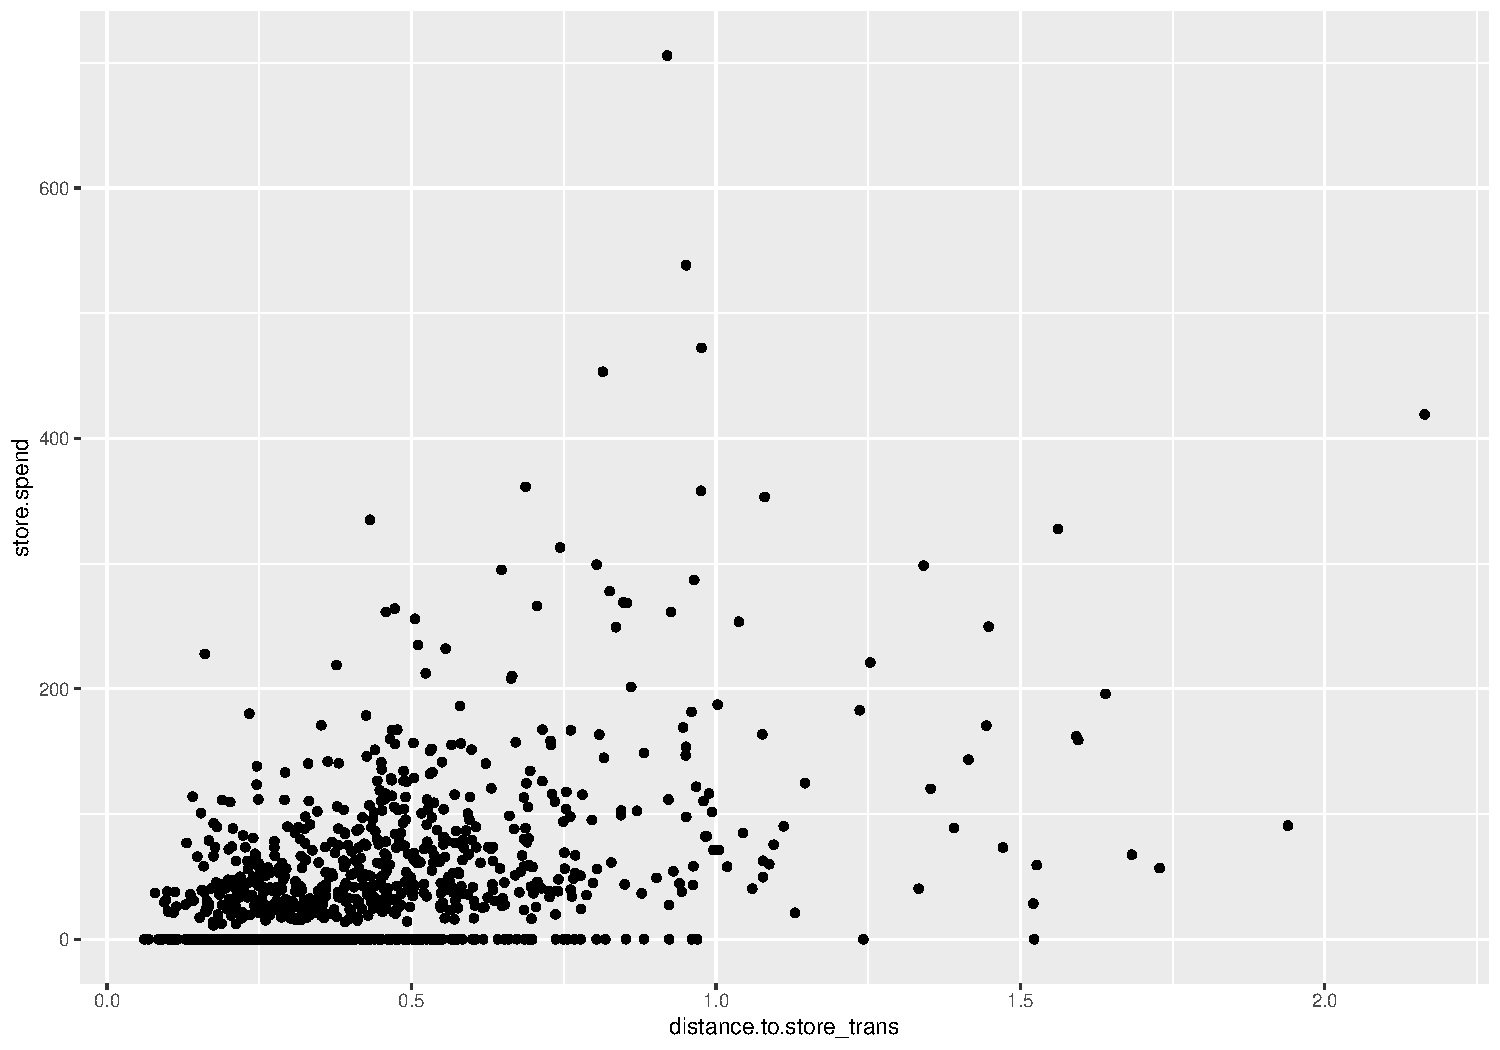
\includegraphics[width=0.5\textwidth,height=\textheight]{004_relationships_between_continuous_variables_files/figure-beamer/unnamed-chunk-22-1.pdf}
\end{center}
\end{frame}

\begin{frame}[fragile]{}
\phantomsection\label{section-23}
\begin{itemize}
\item
  \textbf{Transforming variables}

  \begin{itemize}
  \tightlist
  \item
    Understanding the logic behind inverse square root distance
  \end{itemize}
\end{itemize}

\tiny

\begin{Shaded}
\begin{Highlighting}[]
\FunctionTok{ggplot}\NormalTok{() }\SpecialCharTok{+}
  \FunctionTok{geom\_function}\NormalTok{(}\AttributeTok{fun =} \ControlFlowTok{function}\NormalTok{(x) \{}\DecValTok{1} \SpecialCharTok{/} \FunctionTok{sqrt}\NormalTok{(x)\}) }\SpecialCharTok{+}
  \FunctionTok{labs}\NormalTok{(}\AttributeTok{x =} \StringTok{"Distance"}\NormalTok{,}
       \AttributeTok{y =} \StringTok{"Inverse square root distance"}\NormalTok{)}
\end{Highlighting}
\end{Shaded}

\begin{center}
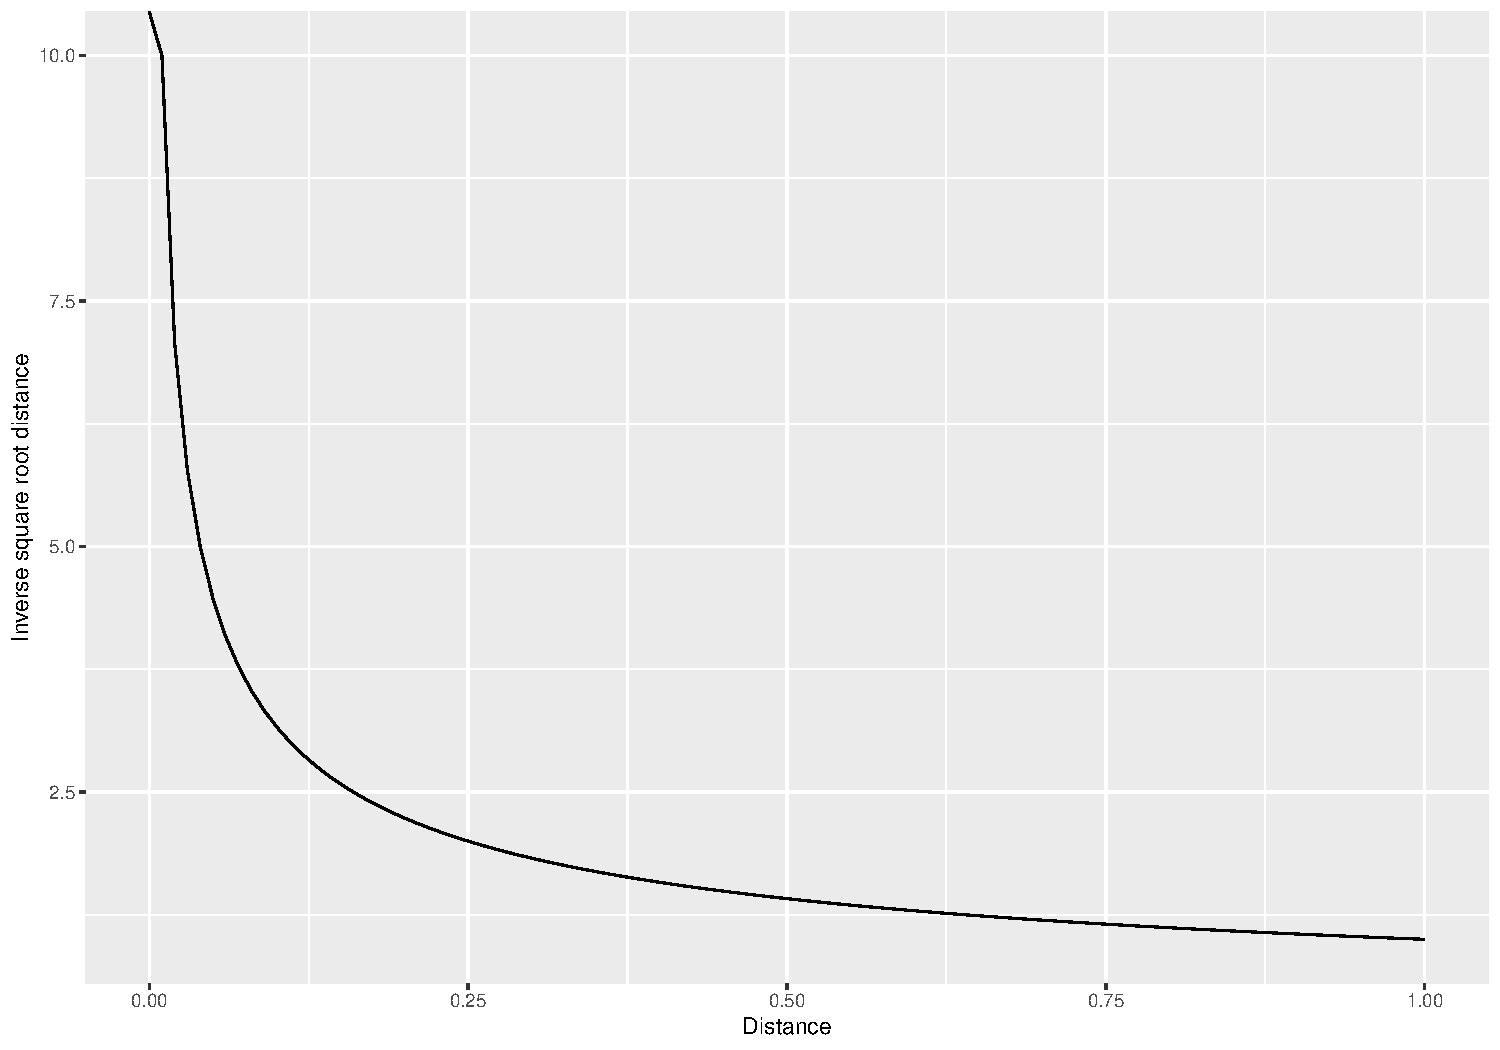
\includegraphics[width=0.5\textwidth,height=\textheight]{004_relationships_between_continuous_variables_files/figure-beamer/unnamed-chunk-23-1.pdf}
\end{center}
\end{frame}

\begin{frame}[fragile]{}
\phantomsection\label{section-24}
\begin{itemize}
\item
  \textbf{Visualizing categorical variables}

  \begin{itemize}
  \tightlist
  \item
    \textbf{Scatterplots: the base R way}
  \end{itemize}
\end{itemize}

\tiny

\begin{Shaded}
\begin{Highlighting}[]
\FunctionTok{plot}\NormalTok{(}\FunctionTok{as.integer}\NormalTok{(customer}\SpecialCharTok{$}\NormalTok{sat.service), }\FunctionTok{as.integer}\NormalTok{(customer}\SpecialCharTok{$}\NormalTok{sat.selection),}
     \AttributeTok{xlab =} \StringTok{"Customer Satisfaction with Service"}\NormalTok{,}
     \AttributeTok{ylab =} \StringTok{"Customer Satisfaction with Selection"}\NormalTok{,}
     \AttributeTok{main =} \StringTok{"Customer as of June 2014"}\NormalTok{)}
\end{Highlighting}
\end{Shaded}

\begin{center}
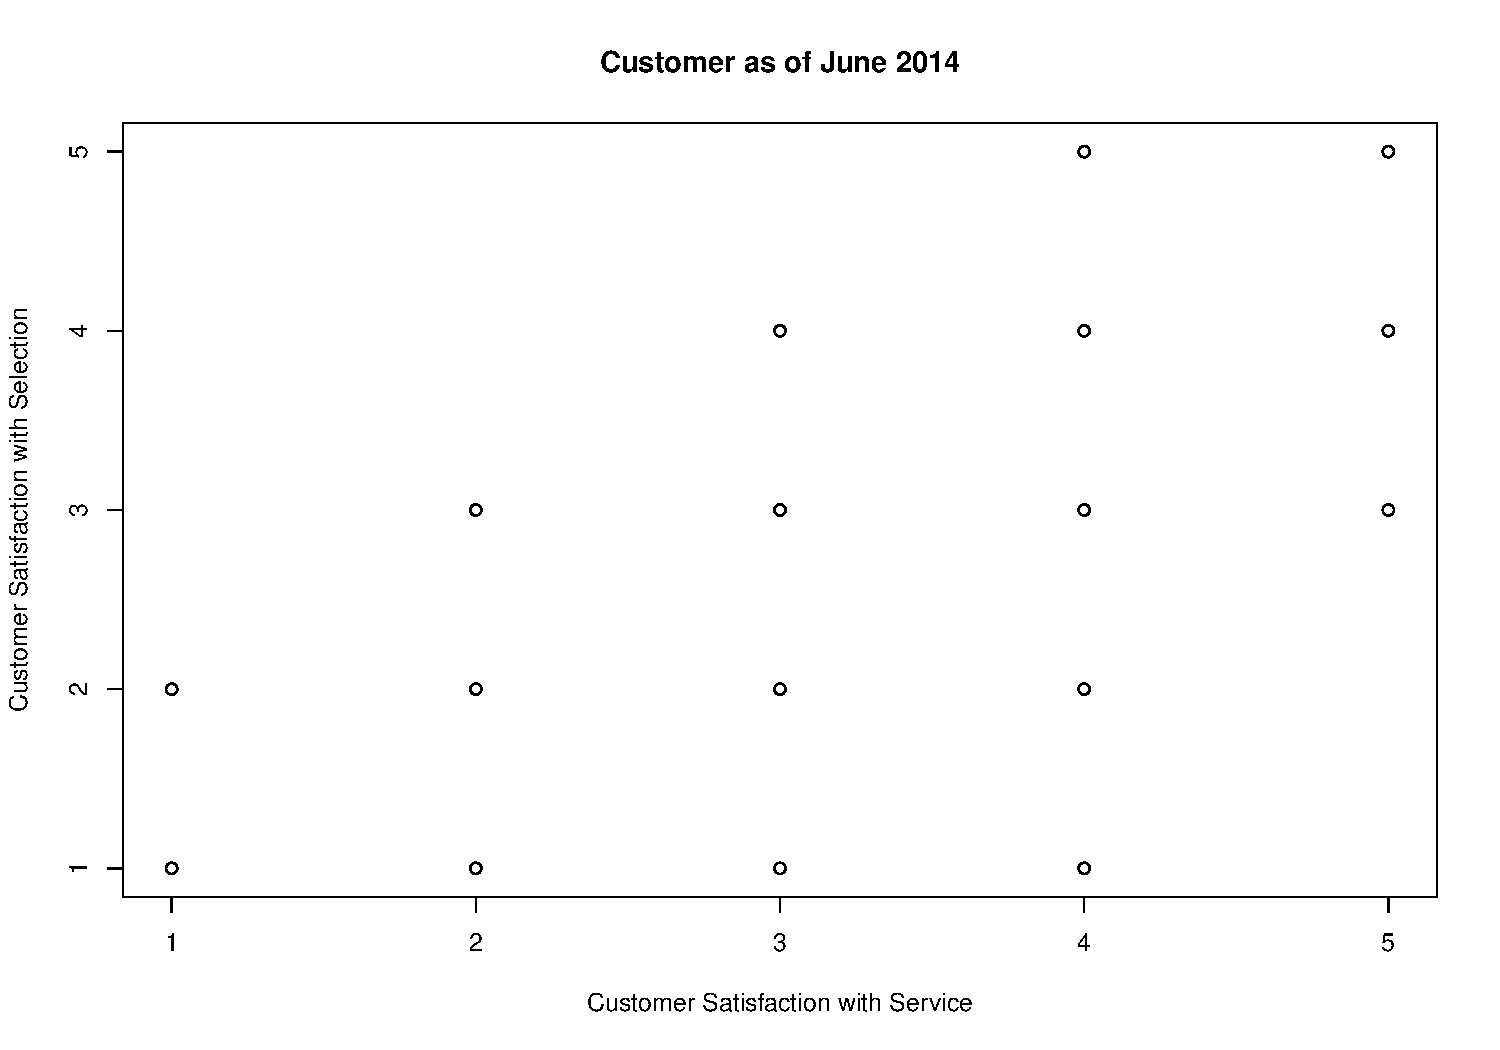
\includegraphics[width=0.5\textwidth,height=\textheight]{004_relationships_between_continuous_variables_files/figure-beamer/unnamed-chunk-24-1.pdf}
\end{center}
\end{frame}

\begin{frame}[fragile]{}
\phantomsection\label{section-25}
\begin{itemize}
\item
  \textbf{Visualizing categorical variables}

  \begin{itemize}
  \tightlist
  \item
    \textbf{Scatterplots: the base R way}
  \end{itemize}
\end{itemize}

\tiny

\begin{Shaded}
\begin{Highlighting}[]
\FunctionTok{plot}\NormalTok{(}\FunctionTok{jitter}\NormalTok{(}\FunctionTok{as.integer}\NormalTok{(customer}\SpecialCharTok{$}\NormalTok{sat.service)), }\FunctionTok{jitter}\NormalTok{(}\FunctionTok{as.integer}\NormalTok{(customer}\SpecialCharTok{$}\NormalTok{sat.selection)),}
     \AttributeTok{xlab =} \StringTok{"Customer Satisfaction with Service"}\NormalTok{,}
     \AttributeTok{ylab =} \StringTok{"Customer Satisfaction with Selection"}\NormalTok{,}
     \AttributeTok{main =} \StringTok{"Customer as of June 2014"}\NormalTok{)}
\end{Highlighting}
\end{Shaded}

\begin{center}
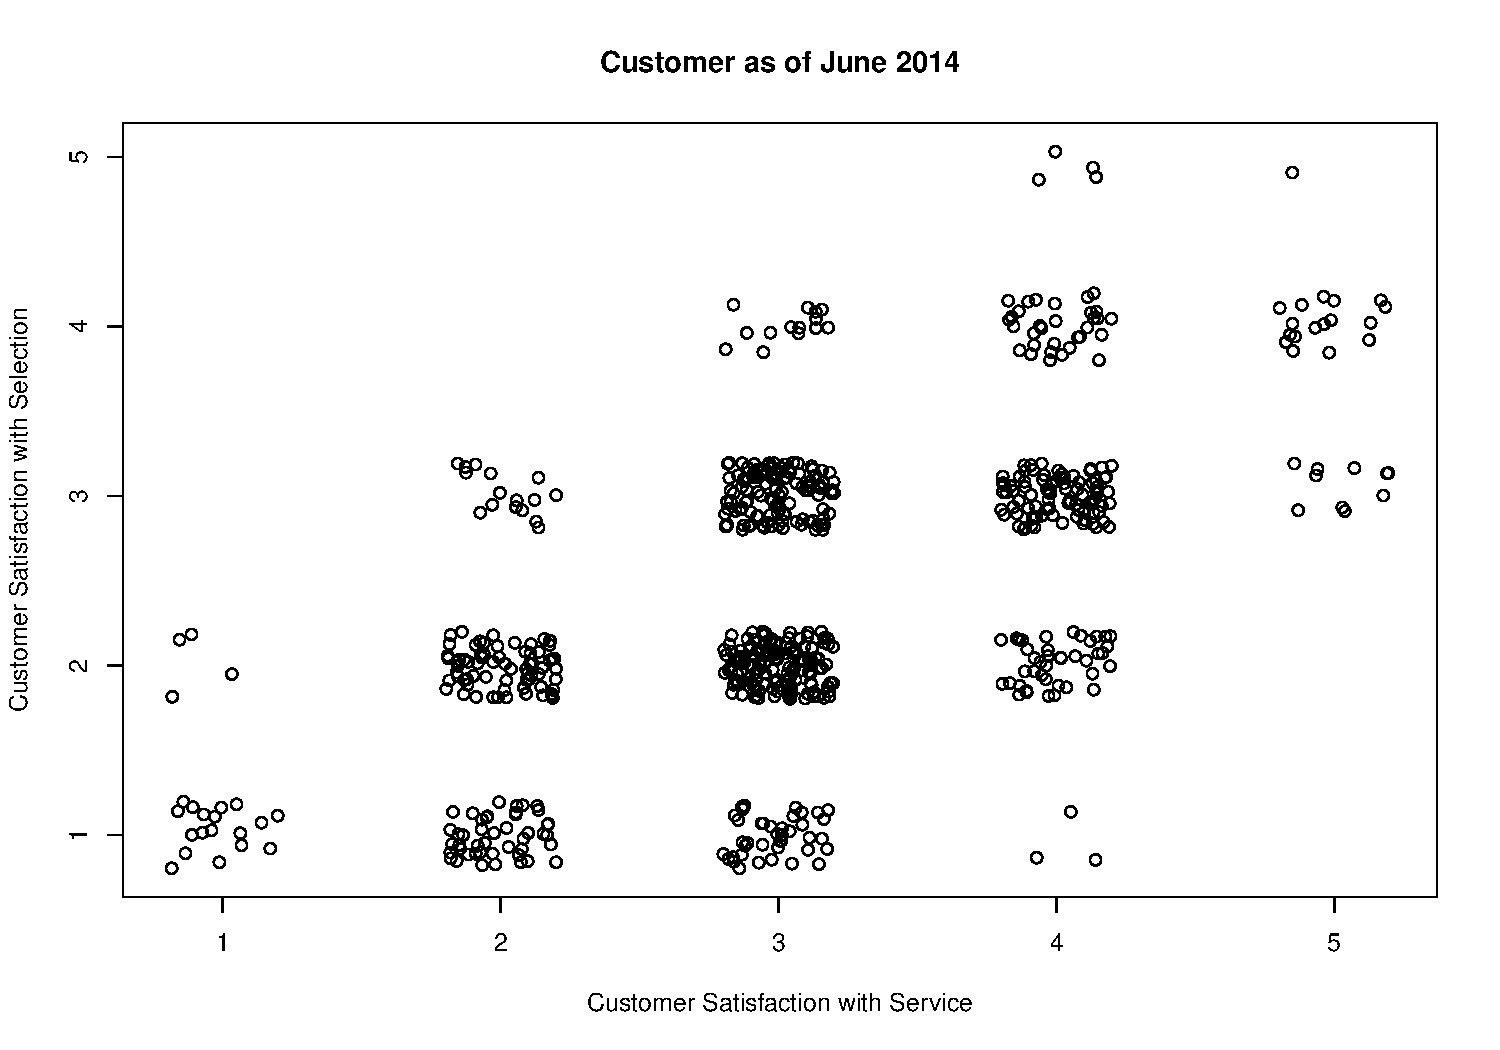
\includegraphics[width=0.5\textwidth,height=\textheight]{004_relationships_between_continuous_variables_files/figure-beamer/unnamed-chunk-25-1.pdf}
\end{center}
\end{frame}

\begin{frame}[fragile]{}
\phantomsection\label{section-26}
\begin{itemize}
\item
  \textbf{Visualizing categorical variables}

  \begin{itemize}
  \tightlist
  \item
    \textbf{Scatterplots: the tidyverse way}
  \end{itemize}
\end{itemize}

\tiny

\begin{Shaded}
\begin{Highlighting}[]
\NormalTok{customer }\SpecialCharTok{|\textgreater{}} 
  \FunctionTok{ggplot}\NormalTok{() }\SpecialCharTok{+}
  \FunctionTok{geom\_point}\NormalTok{(}\FunctionTok{aes}\NormalTok{(}\AttributeTok{x =}\NormalTok{ sat.service, }\AttributeTok{y =}\NormalTok{ sat.selection)) }\SpecialCharTok{+}
  \FunctionTok{labs}\NormalTok{(}\AttributeTok{x =} \StringTok{"Customer Satisfaction with Service"}\NormalTok{,}
       \AttributeTok{y =} \StringTok{"Customer Satisfaction with Selection"}\NormalTok{,}
       \AttributeTok{title =} \StringTok{"Customer as of June 2014"}\NormalTok{)}
\end{Highlighting}
\end{Shaded}

\begin{center}
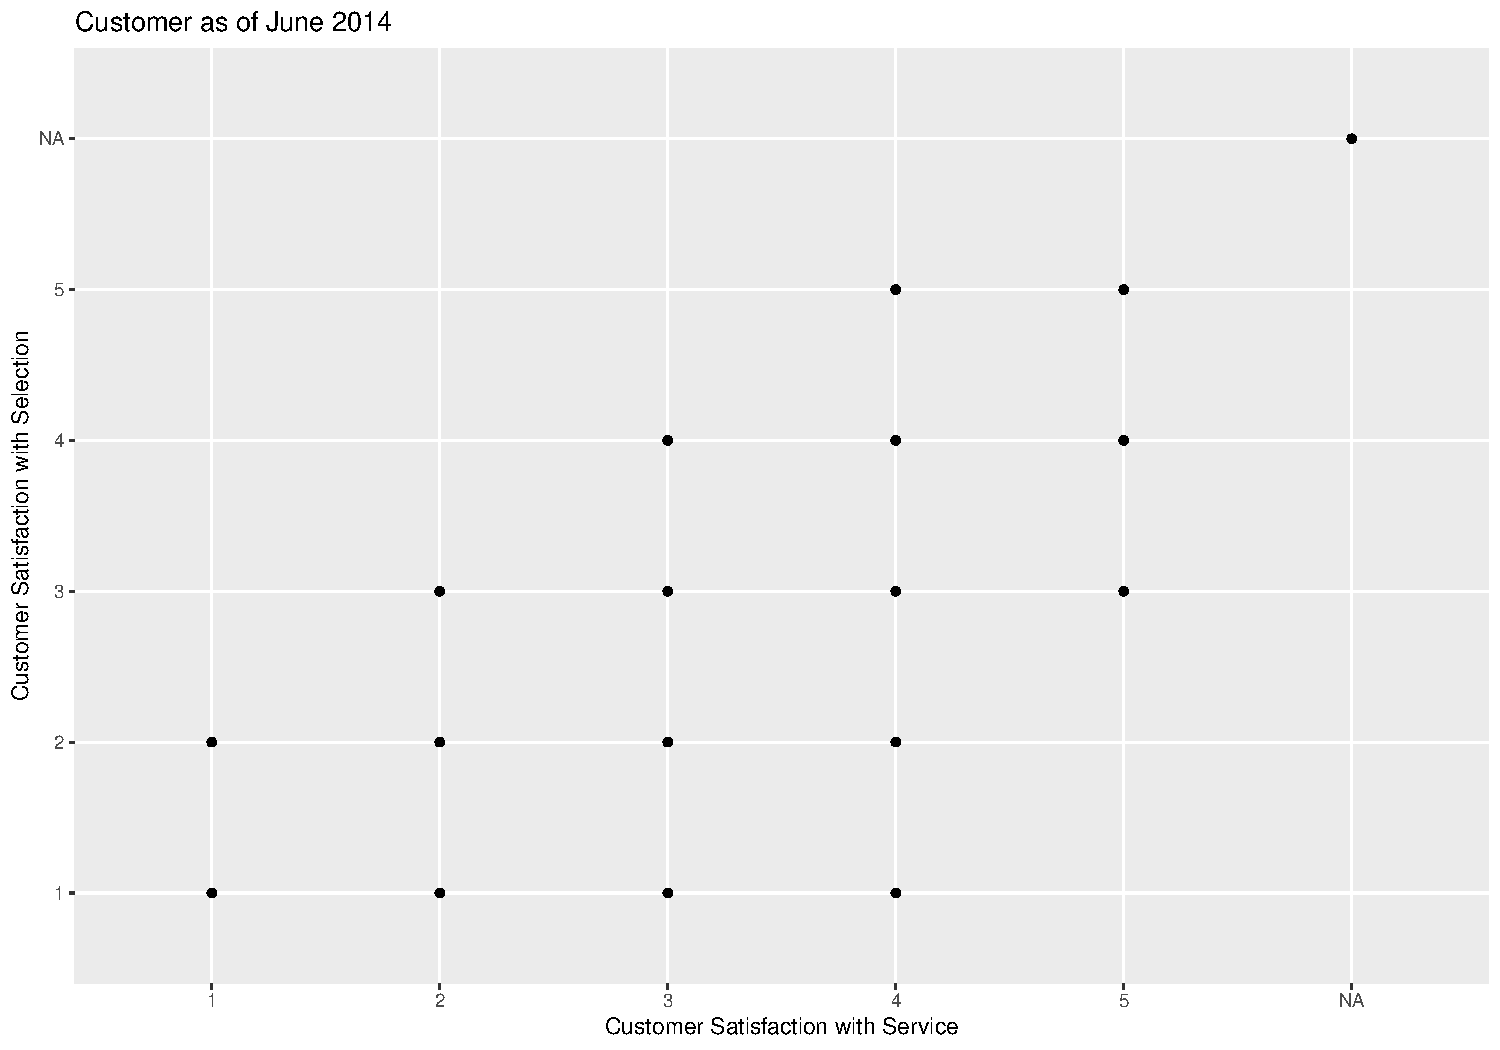
\includegraphics[width=0.5\textwidth,height=\textheight]{004_relationships_between_continuous_variables_files/figure-beamer/unnamed-chunk-26-1.pdf}
\end{center}
\end{frame}

\begin{frame}[fragile]{}
\phantomsection\label{section-27}
\begin{itemize}
\item
  \textbf{Visualizing categorical variables}

  \begin{itemize}
  \tightlist
  \item
    \textbf{Scatterplots: the tidyverse way}
  \end{itemize}
\end{itemize}

\tiny

\begin{Shaded}
\begin{Highlighting}[]
\NormalTok{customer }\SpecialCharTok{|\textgreater{}} 
  \FunctionTok{ggplot}\NormalTok{() }\SpecialCharTok{+}
  \FunctionTok{geom\_point}\NormalTok{(}\FunctionTok{aes}\NormalTok{(}\AttributeTok{x =}\NormalTok{ sat.service, }\AttributeTok{y =}\NormalTok{ sat.selection), }
             \AttributeTok{position =} \FunctionTok{position\_jitter}\NormalTok{(}\AttributeTok{width =} \FloatTok{0.2}\NormalTok{, }\AttributeTok{height =} \FloatTok{0.2}\NormalTok{)) }\SpecialCharTok{+}
  \FunctionTok{labs}\NormalTok{(}\AttributeTok{x =} \StringTok{"Customer Satisfaction with Service"}\NormalTok{,}
       \AttributeTok{y =} \StringTok{"Customer Satisfaction with Selection"}\NormalTok{,}
       \AttributeTok{title =} \StringTok{"Customer as of June 2014"}\NormalTok{)}
\end{Highlighting}
\end{Shaded}

\begin{center}
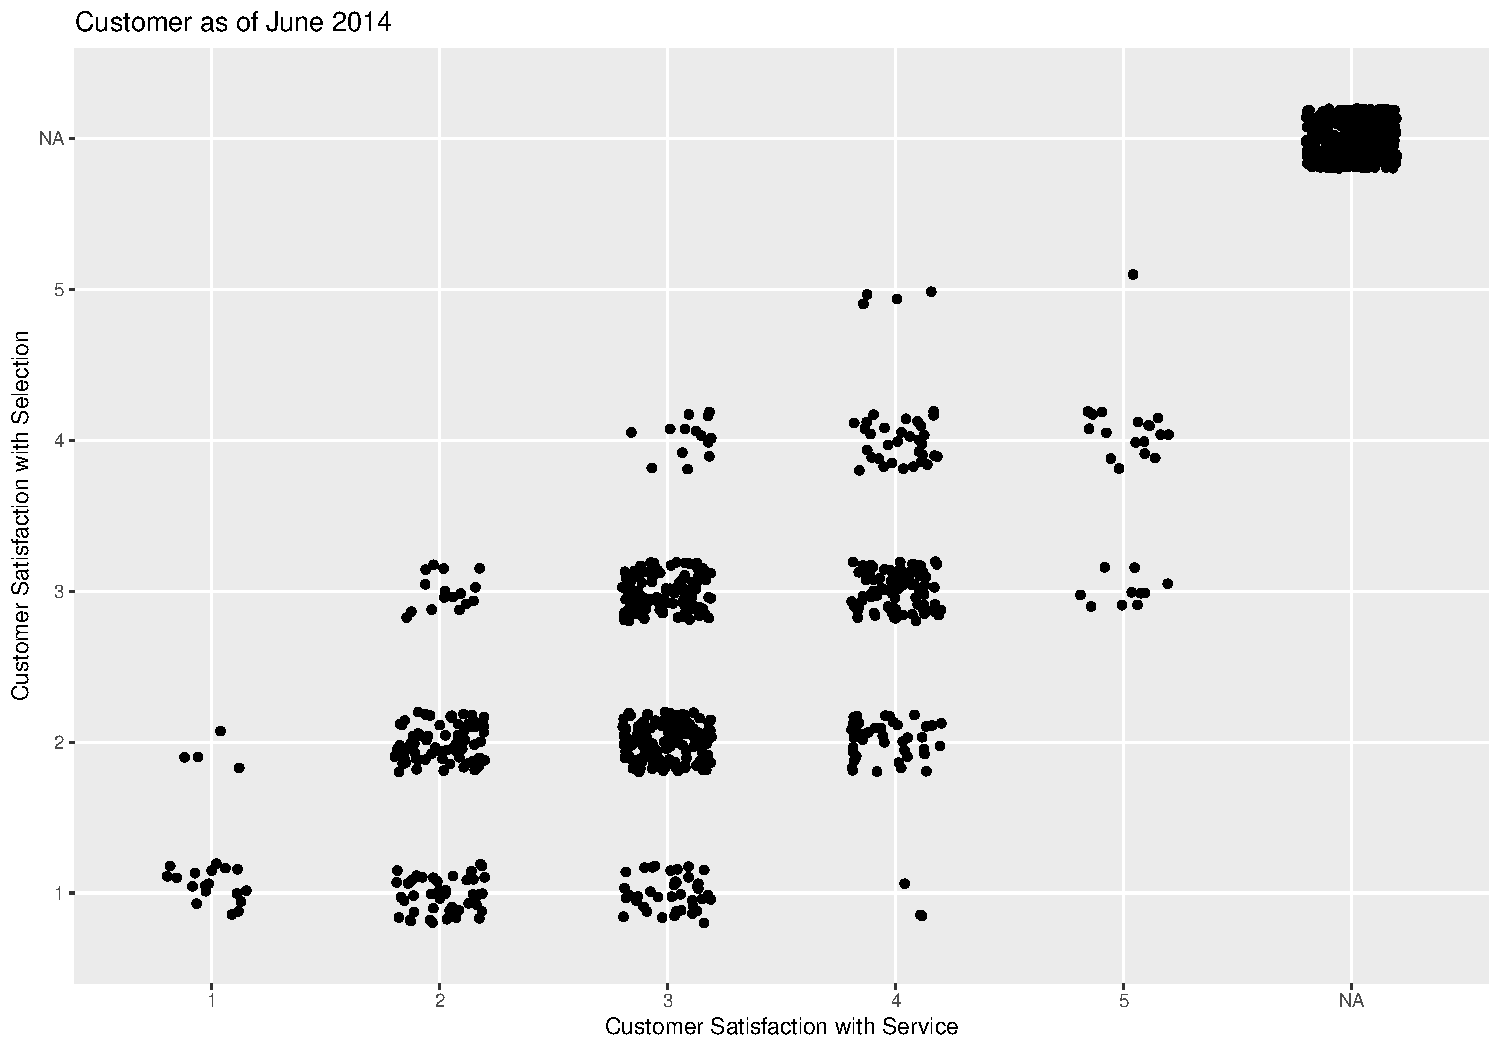
\includegraphics[width=0.5\textwidth,height=\textheight]{004_relationships_between_continuous_variables_files/figure-beamer/unnamed-chunk-27-1.pdf}
\end{center}
\end{frame}

\section{Acknowledgments}\label{acknowledgments}

\begin{frame}{}
\phantomsection\label{section-28}
\begin{itemize}
\item
  To my family that supports me
\item
  To the taxpayers of Colombia and the
  \href{https://www.umng.edu.co/estudiante}{\textbf{UMNG students}} who
  pay my salary
\item
  To the \href{https://www.business-science.io/}{\textbf{Business
  Science}} and \href{https://www.rfordatasci.com/}{\textbf{R4DS Online
  Learning}} communities where I learn
  \href{https://www.r-project.org/about.html}{\textbf{R}} and
  \href{https://www.python.org/about/}{\textbf{\(\pi\)-thon}}
\item
  To the \href{https://www.r-project.org/contributors.html}{\textbf{R
  Core Team}}, the creators of
  \href{https://posit.co/products/open-source/rstudio/}{\textbf{RStudio
  IDE}}, \href{https://quarto.org/}{\textbf{Quarto}} and the authors and
  maintainers of the packages
  \href{https://CRAN.R-project.org/package=tidyverse}{\textbf{tidyverse}},
  \href{https://CRAN.R-project.org/package=skimr}{\textbf{skimr}},
  \href{https://CRAN.R-project.org/package=corrr}{\textbf{corrr}} and
  \href{https://CRAN.R-project.org/package=tinytex}{\textbf{tinytex}}
  for allowing me to access these tools without paying for a license
\item
  To the \href{https://www.kernel.org/category/about.html}{\textbf{Linux
  kernel community}} for allowing me the possibility to use some
  \href{https://static.lwn.net/Distributions/}{\textbf{Linux
  distributions}} as my main
  \href{https://en.wikipedia.org/wiki/Operating_system}{\textbf{OS}}
  without paying for a license
\end{itemize}
\end{frame}

\section*{References}\label{references}
\addcontentsline{toc}{section}{References}

\begin{frame}{References}
\phantomsection\label{refs}
\begin{CSLReferences}{1}{0}
\bibitem[\citeproctext]{ref-chapman_r_2019}
Chapman, Chris, and Elea McDonnell Feit. 2019. \emph{R {For} {Marketing}
{Research} and {Analytics}}. 2nd ed. 2019. Use {R}! Cham: Springer
International Publishing : Imprint: Springer.
\url{https://doi-org.ezproxy.umng.edu.co/10.1007/978-3-030-14316-9}.

\end{CSLReferences}
\end{frame}




\end{document}
